
\clearpage
\cleardoublepage

\chapter{Experiments \& Results}

The experimentation is conducted on four different types of map projections, namely Cylindrical, Pseudocylindrical, Conic and Planar projections. Each of the map projections type contain four different map projections.
The U-Net model mentioned in \autoref{chap:approach} is trained for 20 epochs for each of the map projections. Initially 120 epochs were defined for the experimentation, for each of the models the phenomenon of overfitting started to occur over the training period, to mitigate the issue \textbf{early stopping} was deployed and each model was trained for 20 epochs.
Mean absolute error (MAE) is used as a metric for the evaluation of the model.

16 datasets were generated for the experimentation, via the process of creating rasters as mentioned in \autoref{chap:preprocess}. The loss and the metrics discussed in the result section are the average results, as for each map projection dataset the U-Net model is trained four times mitigating the issue of randomness in the networks parameters.
\section{Cylindrical Projections}
The four cylindrical map projections used for the expertimention are Mercator, Plate Carree, Cylindrical Equal Area, and General Oblique Transformation. The selection of the map projections in done based on the underlying properties of the cylindrical map projections.

\subsubsection*{Mercator}
\begin{figure}[h]
    \centering
    \begin{minipage}{0.30\textwidth}
        \centering
        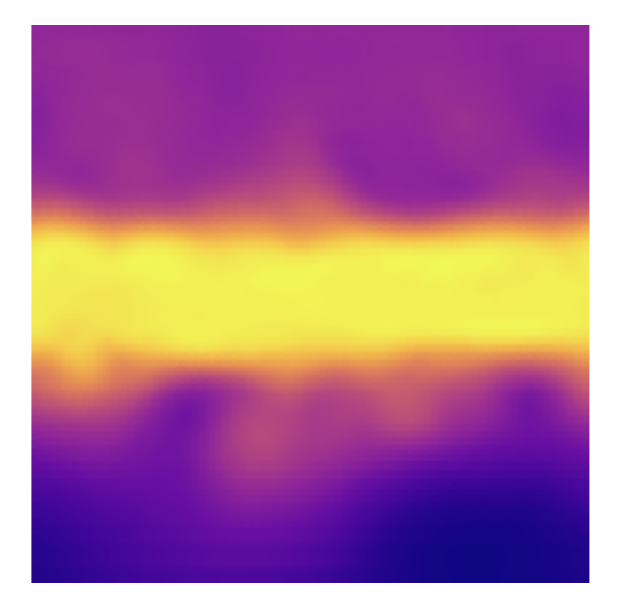
\includegraphics[width=0.9\linewidth]{figures/chapter-8/geopoth_mercator.png}
        \caption{ Geopotential height raster data as Mercator projected}
        \label{fig:merc_geopoth_raster}
    \end{minipage}\hfill
    \begin{minipage}{0.30\textwidth}
        \centering
        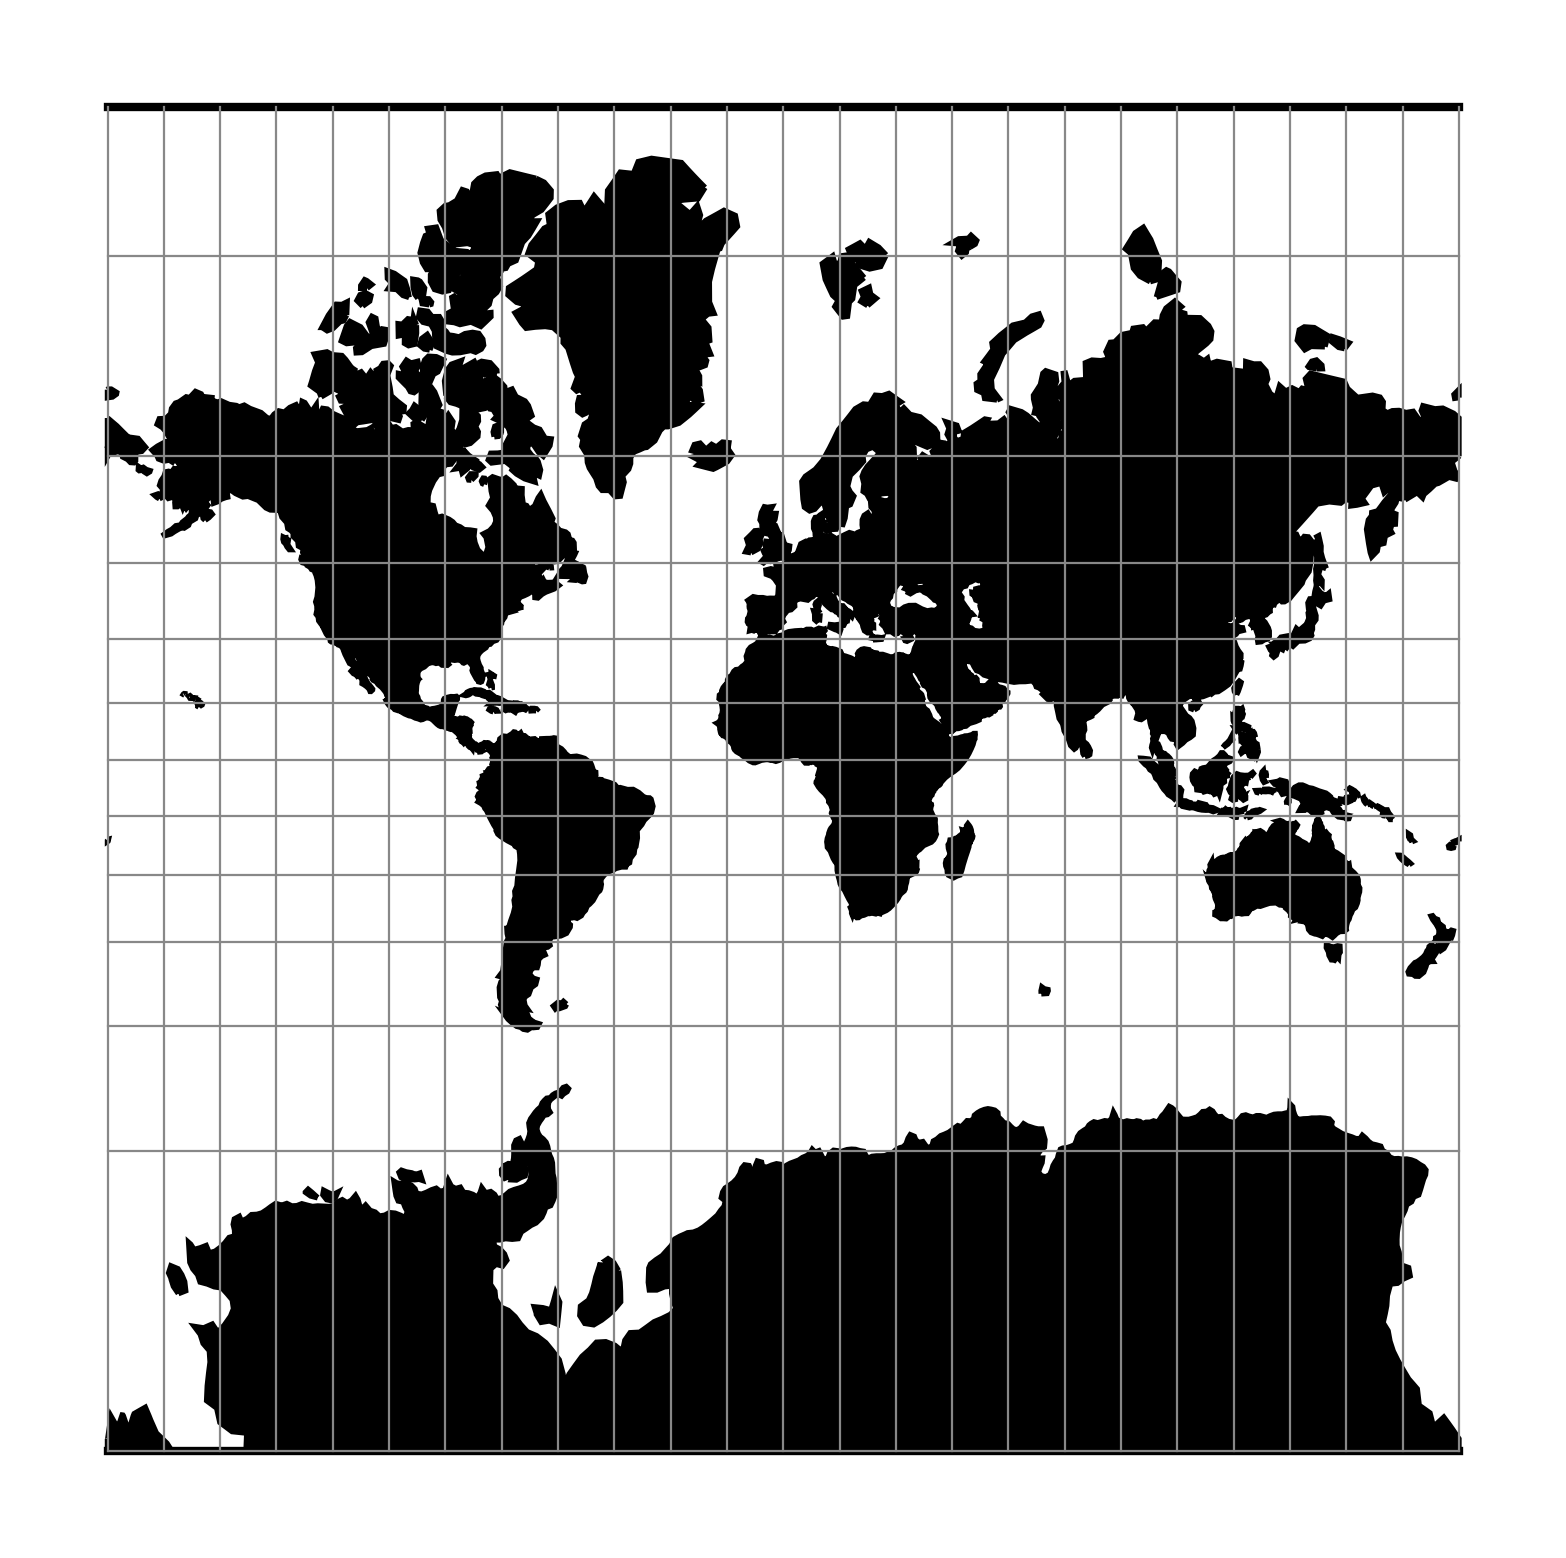
\includegraphics[width=0.9\linewidth]{figures/chapter-8/merc.png}
        \caption{Mercator Projection (Source \cite{PROJ_SITE})}
        \label{fig:merc_proj}
    \end{minipage}\hfill
    \begin{minipage}{0.30\textwidth}
        \centering
        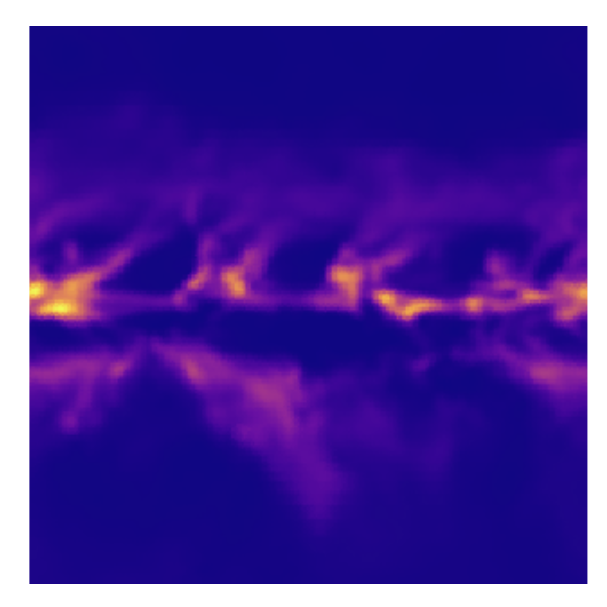
\includegraphics[width=0.9\linewidth]{figures/chapter-8/prect_mercator.png}
        \caption{Precipitation raster data as Mercator projected}
        \label{fig:merc_prect_raster}
    \end{minipage}\hfill
\end{figure}

\begin{figure}[h]
    \centering
    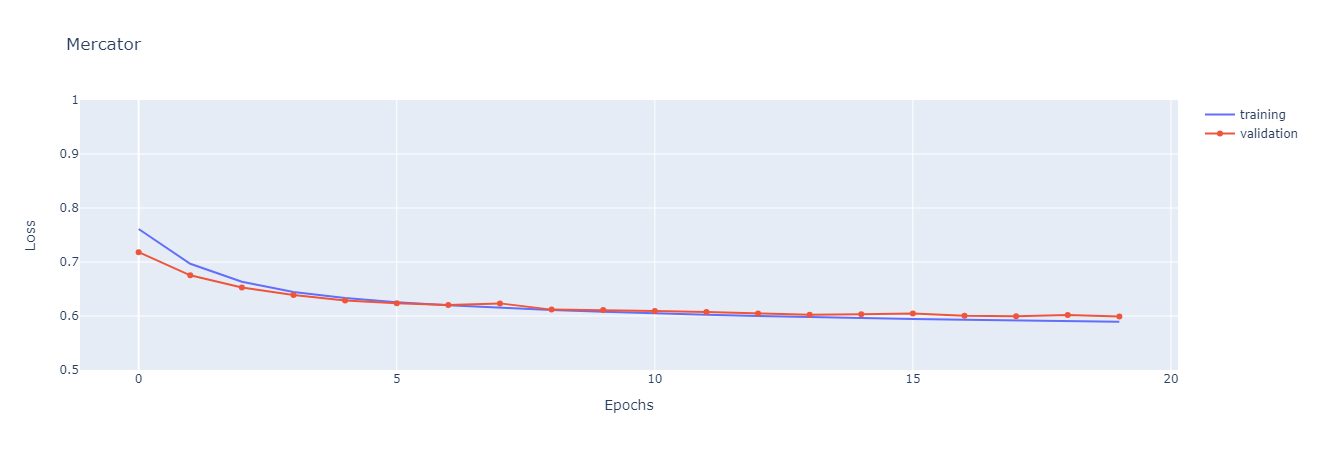
\includegraphics[width=1.0\linewidth]{figures/chapter-8/merc_loss.png}
    \caption{Mercator: Averaged training loss of models  }
    \label{fig:merc_loss}
\end{figure}

\newpage

\subsubsection*{Plate Carree}

\begin{figure}[h]
    \centering
    \begin{minipage}{0.30\textwidth}
        \centering
        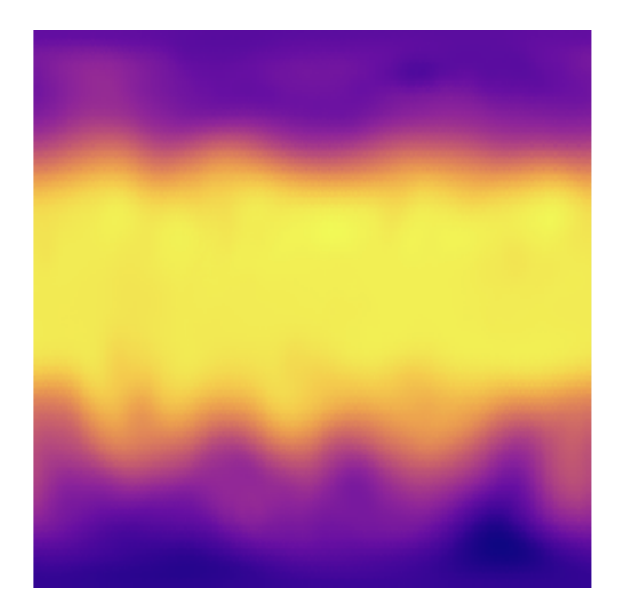
\includegraphics[width=0.9\linewidth]{figures/chapter-8/plate_caree_geopoth_raster.png}
        \caption{ Geopotential height raster data as Plate Carree projected}
        \label{fig:eqc_geopoth_raster}
    \end{minipage}\hfill
    \begin{minipage}{0.30\textwidth}
        \centering
        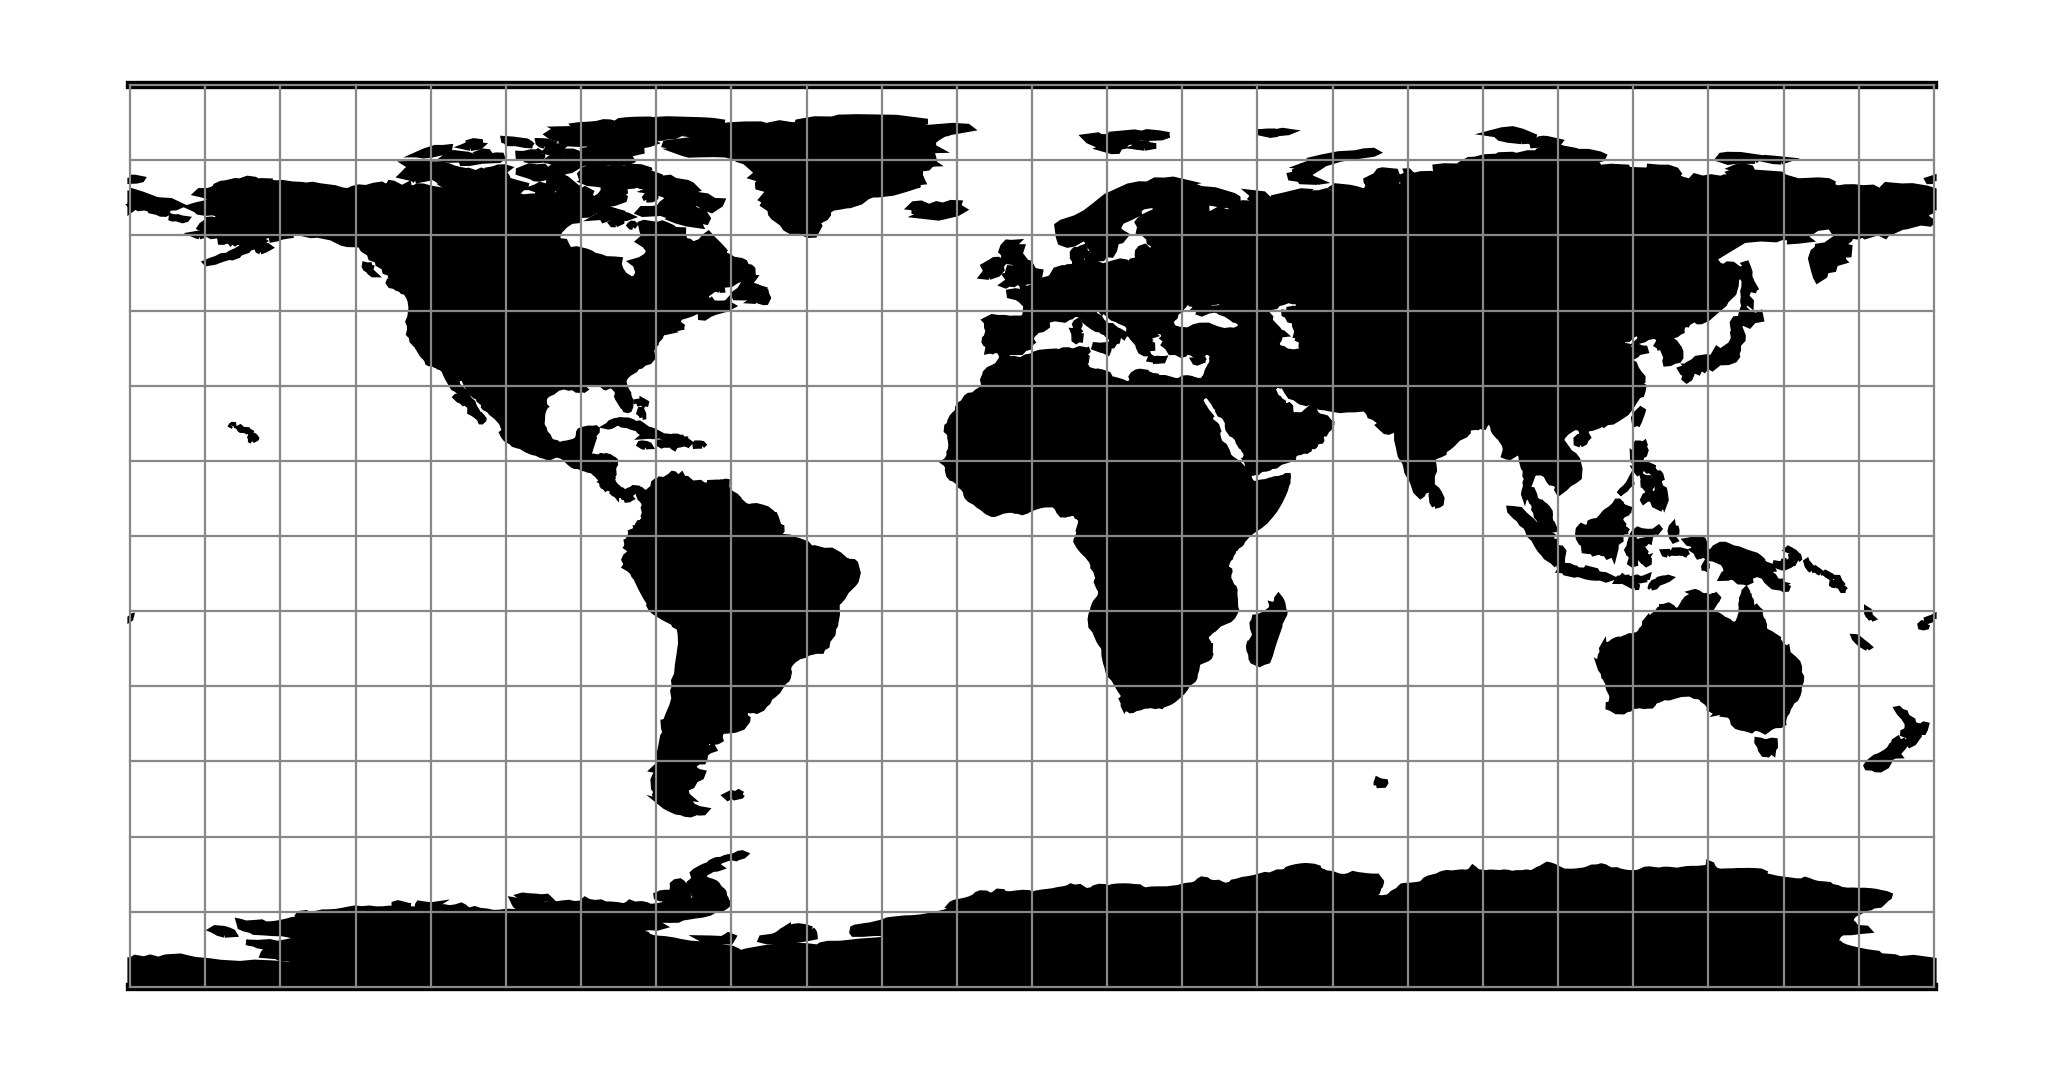
\includegraphics[width=0.9\linewidth]{figures/chapter-8/eqc.png}
        \caption{Plate Carree Projection (Source \cite{PROJ_SITE})}
        \label{fig:eqc_prect_raster}
    \end{minipage}\hfill
    \begin{minipage}{0.30\textwidth}
        \centering
        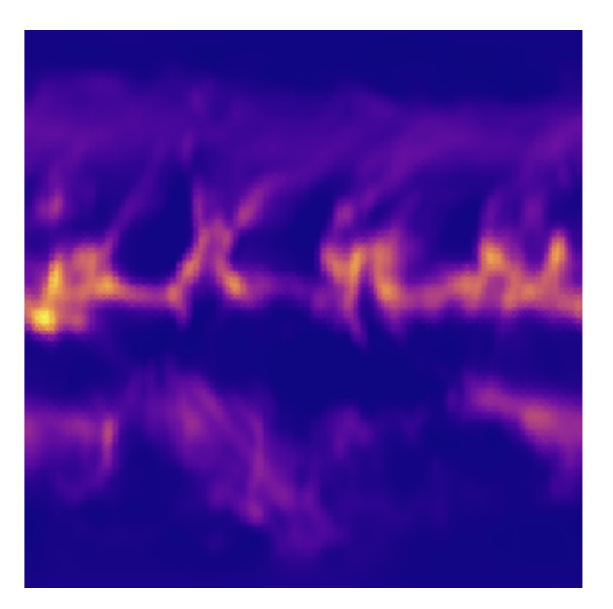
\includegraphics[width=0.9\linewidth]{figures/chapter-8/plate_caree_prect_raster.png}
        \caption{Precipitation raster data as Plate Carree projected}
        \label{fig:eqc_prect_raster}
    \end{minipage}\hfill
\end{figure}

\begin{figure}[h]
    \centering
    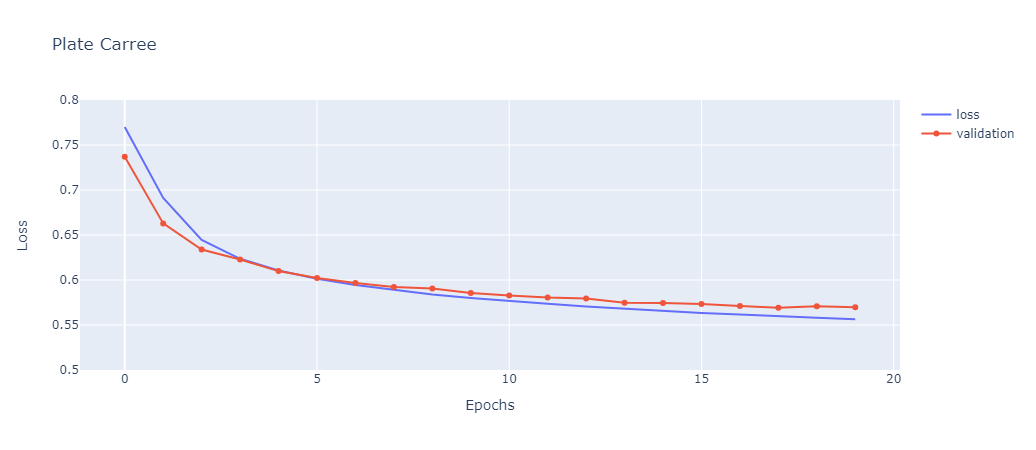
\includegraphics[width=1.0\linewidth]{figures/chapter-8/pc_loss.png}
    \caption{Plate Carree: Averaged training loss of models  }
    \label{fig:pc_loss}
\end{figure}


\subsubsection*{Cylindrical Equal Area}

\begin{figure}[h]
    \centering
    \begin{minipage}{0.30\textwidth}
        \centering
        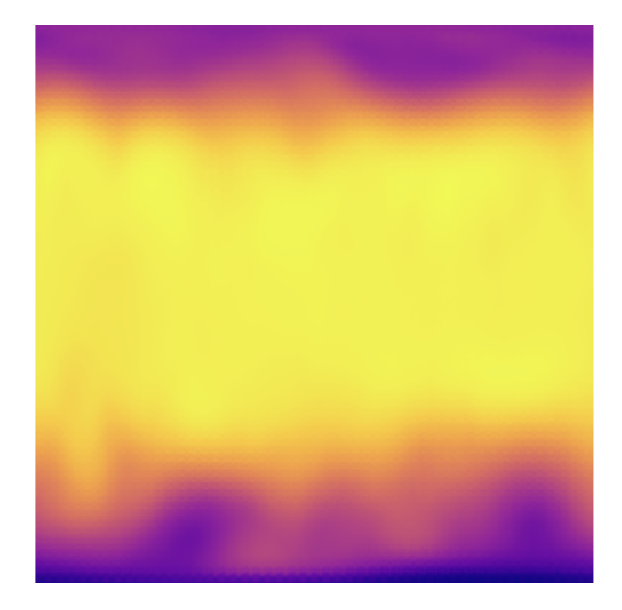
\includegraphics[width=0.9\linewidth]{figures/chapter-8/prect_cea.png}
        \caption{ Geopotential height raster data as Cylindrical Equal Area projected}
        \label{fig:cea_geopoth_raster}
    \end{minipage}\hfill
    \begin{minipage}{0.30\textwidth}
        \centering
        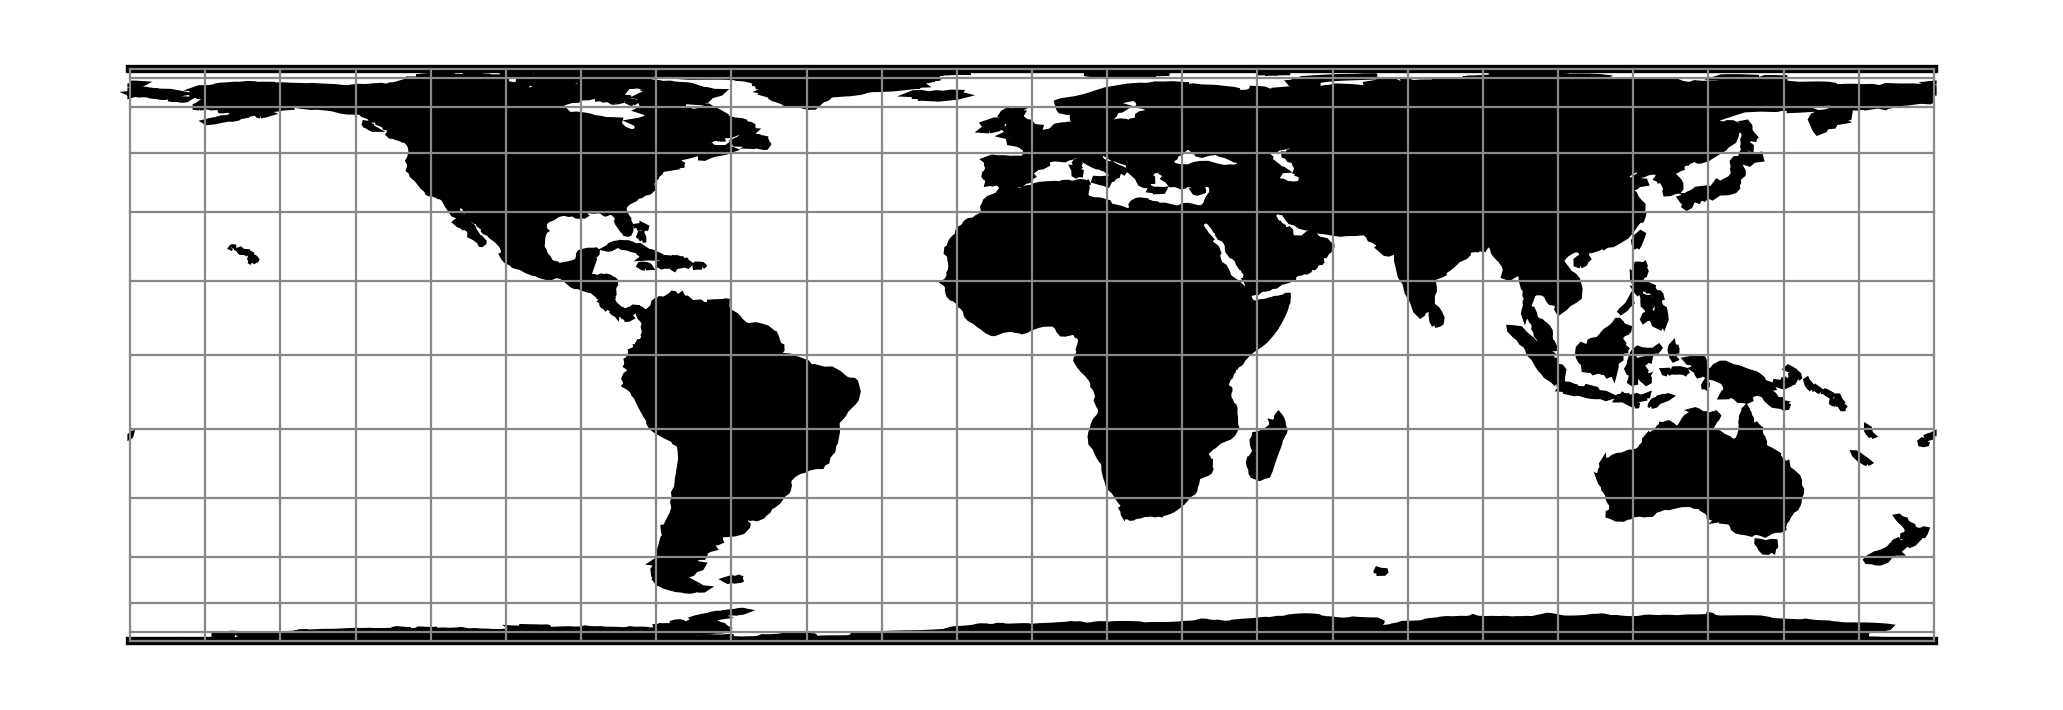
\includegraphics[width=0.9\linewidth]{figures/chapter-8/cea.png}
        \caption{Cylindrical Equal Area Projection (Source \cite{PROJ_SITE})}
        \label{fig:cea_prect_raster}
    \end{minipage}\hfill
    \begin{minipage}{0.30\textwidth}
        \centering
        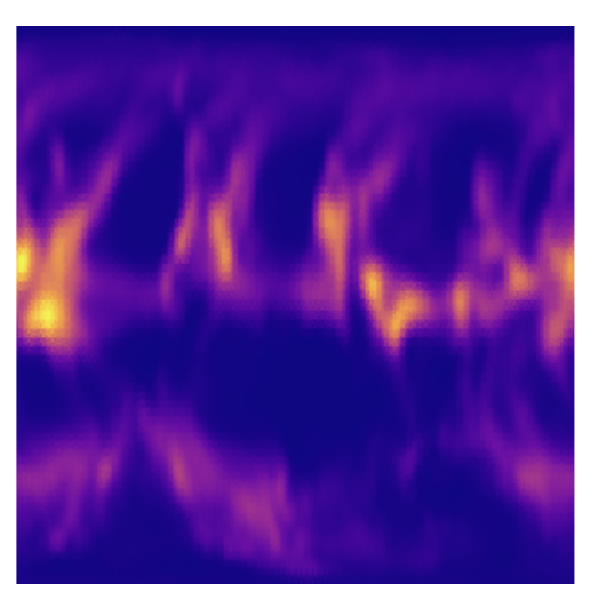
\includegraphics[width=0.9\linewidth]{figures/chapter-8/geopoth_cea.png}
        \caption{Precipitation raster data as Cylindrical Equal Area projected}
        \label{fig:cea_prect_raster}
    \end{minipage}\hfill
\end{figure}

\begin{figure}[h]
    \centering
    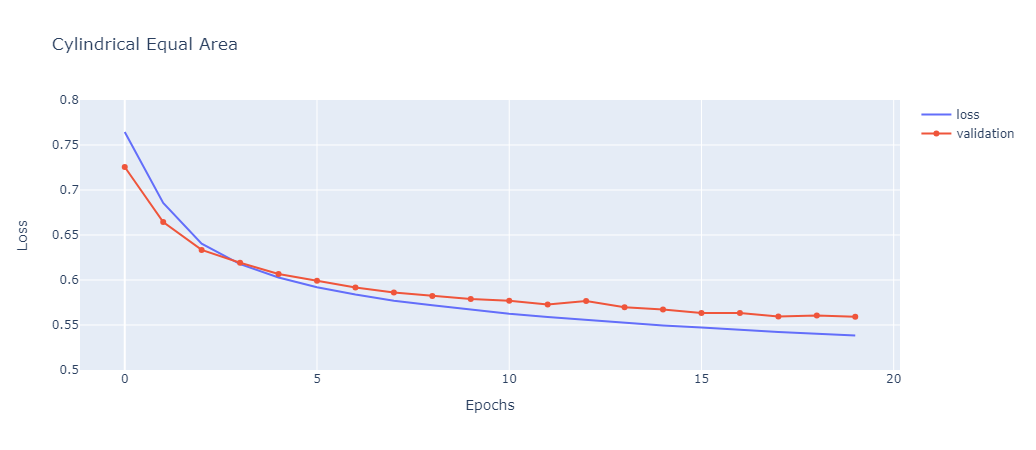
\includegraphics[width=1.0\linewidth]{figures/chapter-8/cea_loss.png}
    \caption{Cylindrical Equal Area: Averaged training loss of models  }
    \label{fig:cea_loss}
\end{figure}

\subsubsection*{General Oblique Transformation}
\begin{figure}[h]
    \centering
    \begin{minipage}{0.30\textwidth}
        \centering
        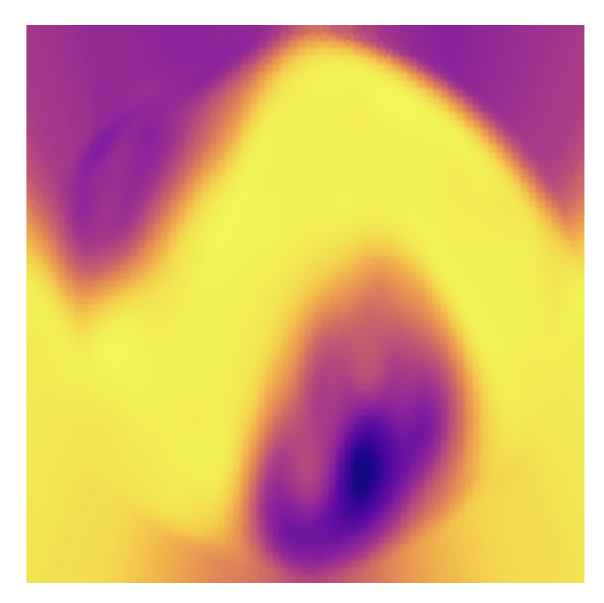
\includegraphics[width=0.9\linewidth]{figures/chapter-8/geopoth_got.png}
        \caption{ Geopotential height raster data as General Oblique Transformation projected}
        \label{fig:ob_tran_geopoth_raster}
    \end{minipage}\hfill
    \begin{minipage}{0.30\textwidth}
        \centering
        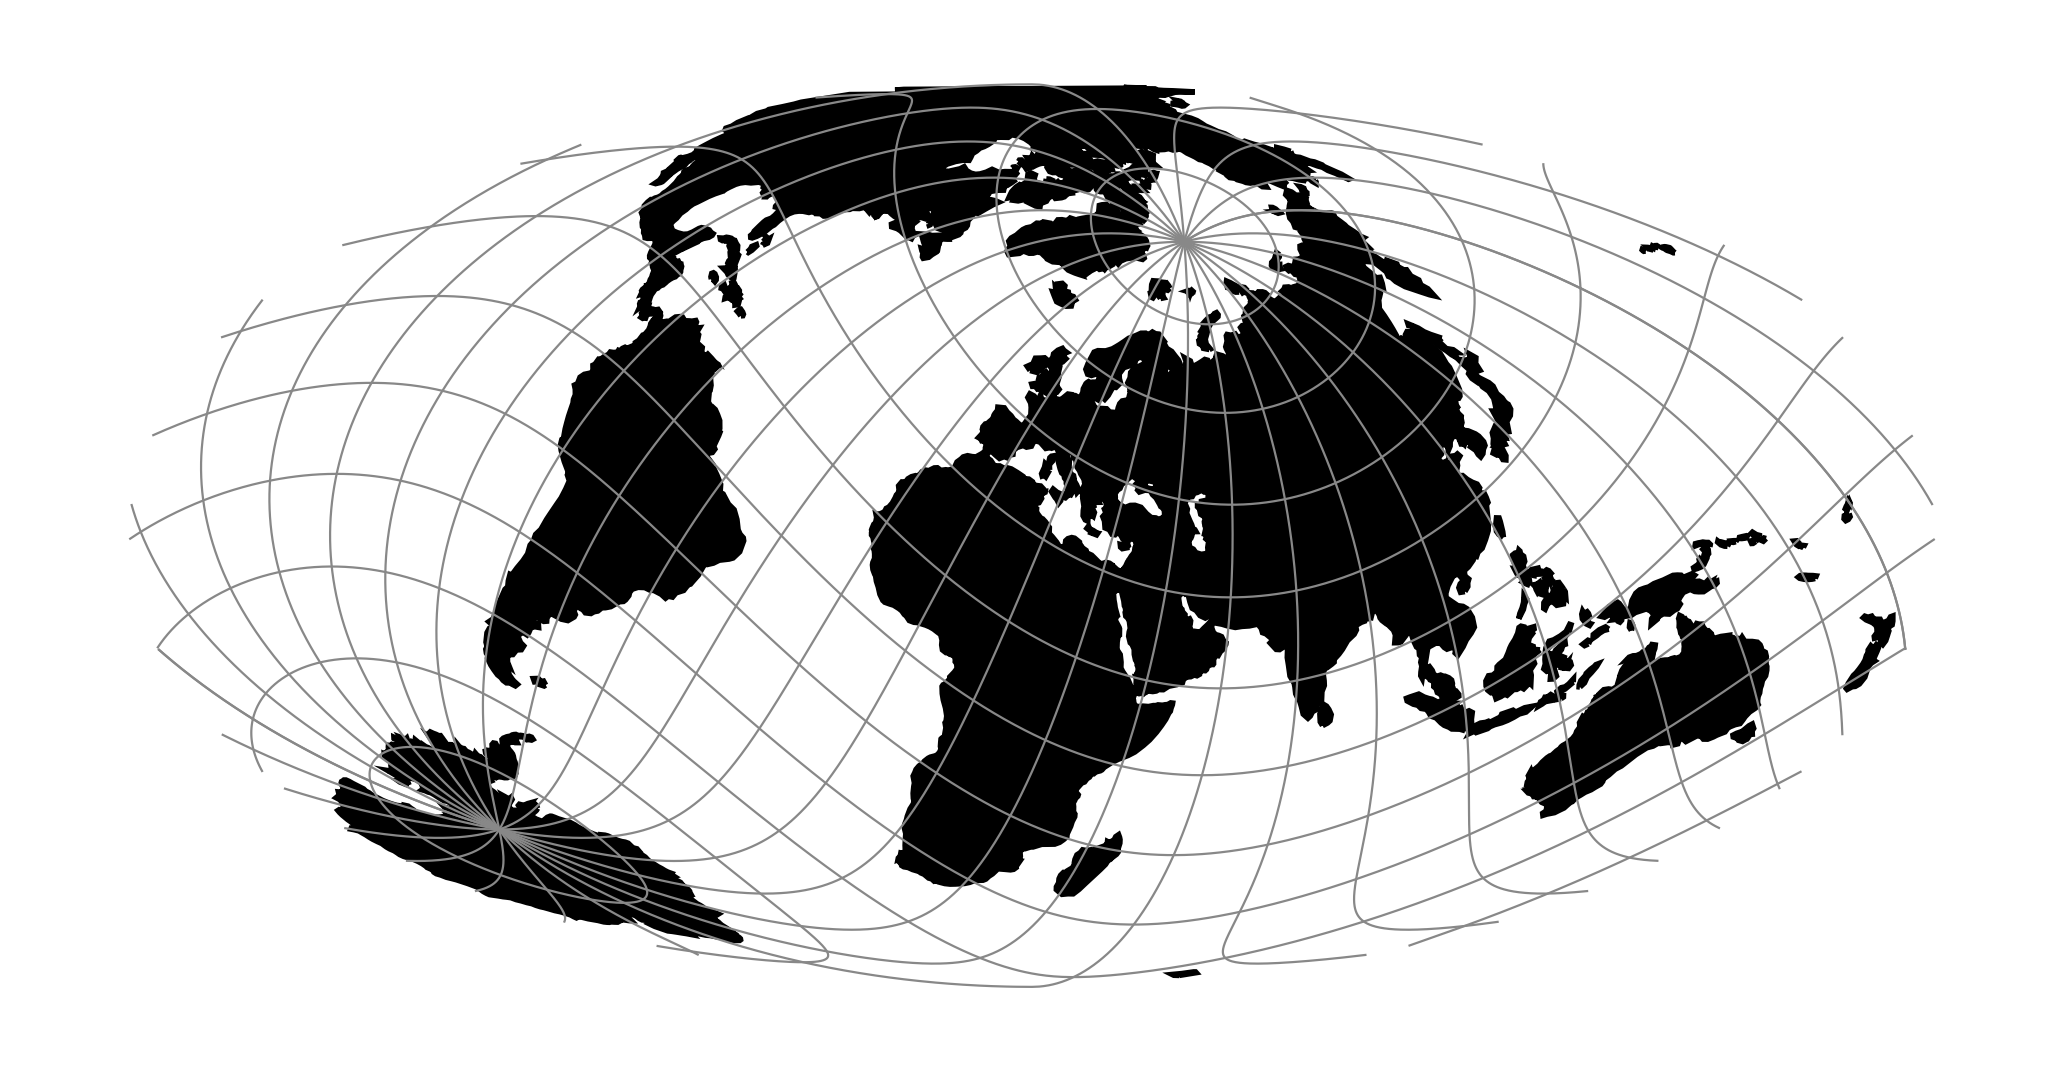
\includegraphics[width=0.9\linewidth]{figures/chapter-8/ob_tran.png}
        \caption{General Oblique Transformation Projection (Source \cite{PROJ_SITE})}
        \label{fig:ob_tran_proj}
    \end{minipage}\hfill
    \begin{minipage}{0.30\textwidth}
        \centering
        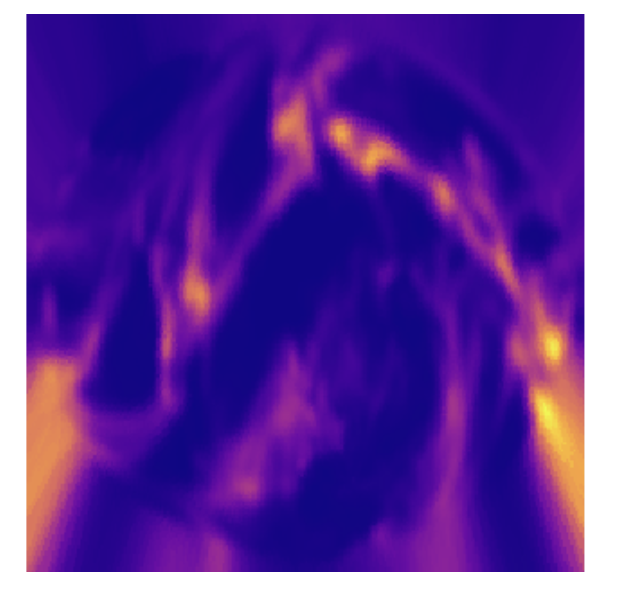
\includegraphics[width=0.9\linewidth]{figures/chapter-8/prect_got.png}
        \caption{Precipitation raster data as General Oblique Transformation projected}
        \label{fig:ob_tran_prect_raster}
    \end{minipage}\hfill
\end{figure}

\begin{figure}[h]
    \centering
    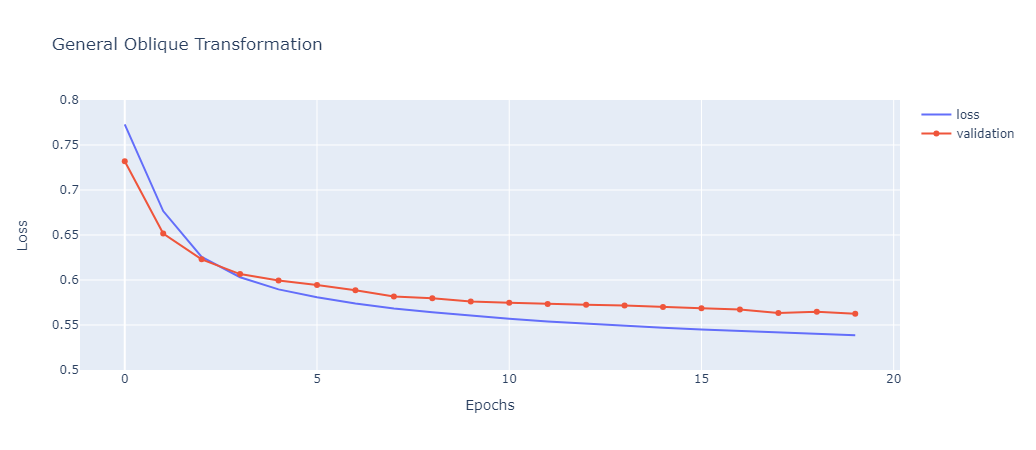
\includegraphics[width=1.0\linewidth]{figures/chapter-8/got_loss.png}
    \caption{General Oblique Transformation: Averaged training loss of models  }
    \label{fig:got_loss}
\end{figure}
\subsection{Results}

\newpage
\section{PseudoCylindrical projections}
\subsubsection*{Robinson}
\begin{figure}[h]
    \centering
    \begin{minipage}{0.30\textwidth}
        \centering
        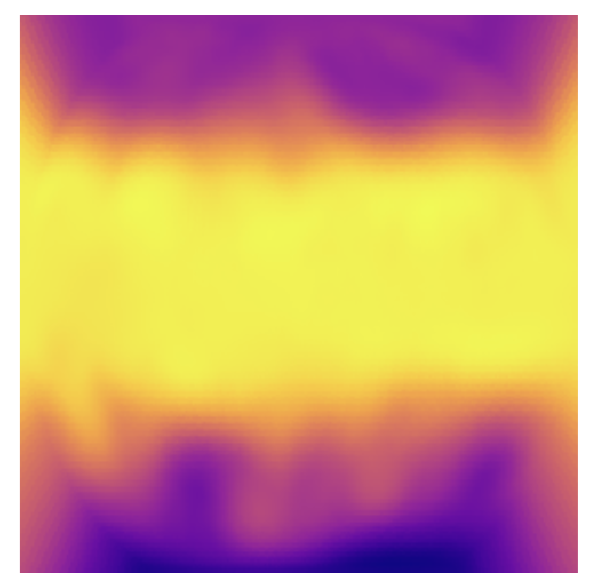
\includegraphics[width=0.9\linewidth]{figures/chapter-8/geopoth_robin.png}
        \caption{ Geopotential height raster data as Robinson projected}
        \label{fig:robin_geopoth_raster}
    \end{minipage}\hfill
    \begin{minipage}{0.30\textwidth}
        \centering
        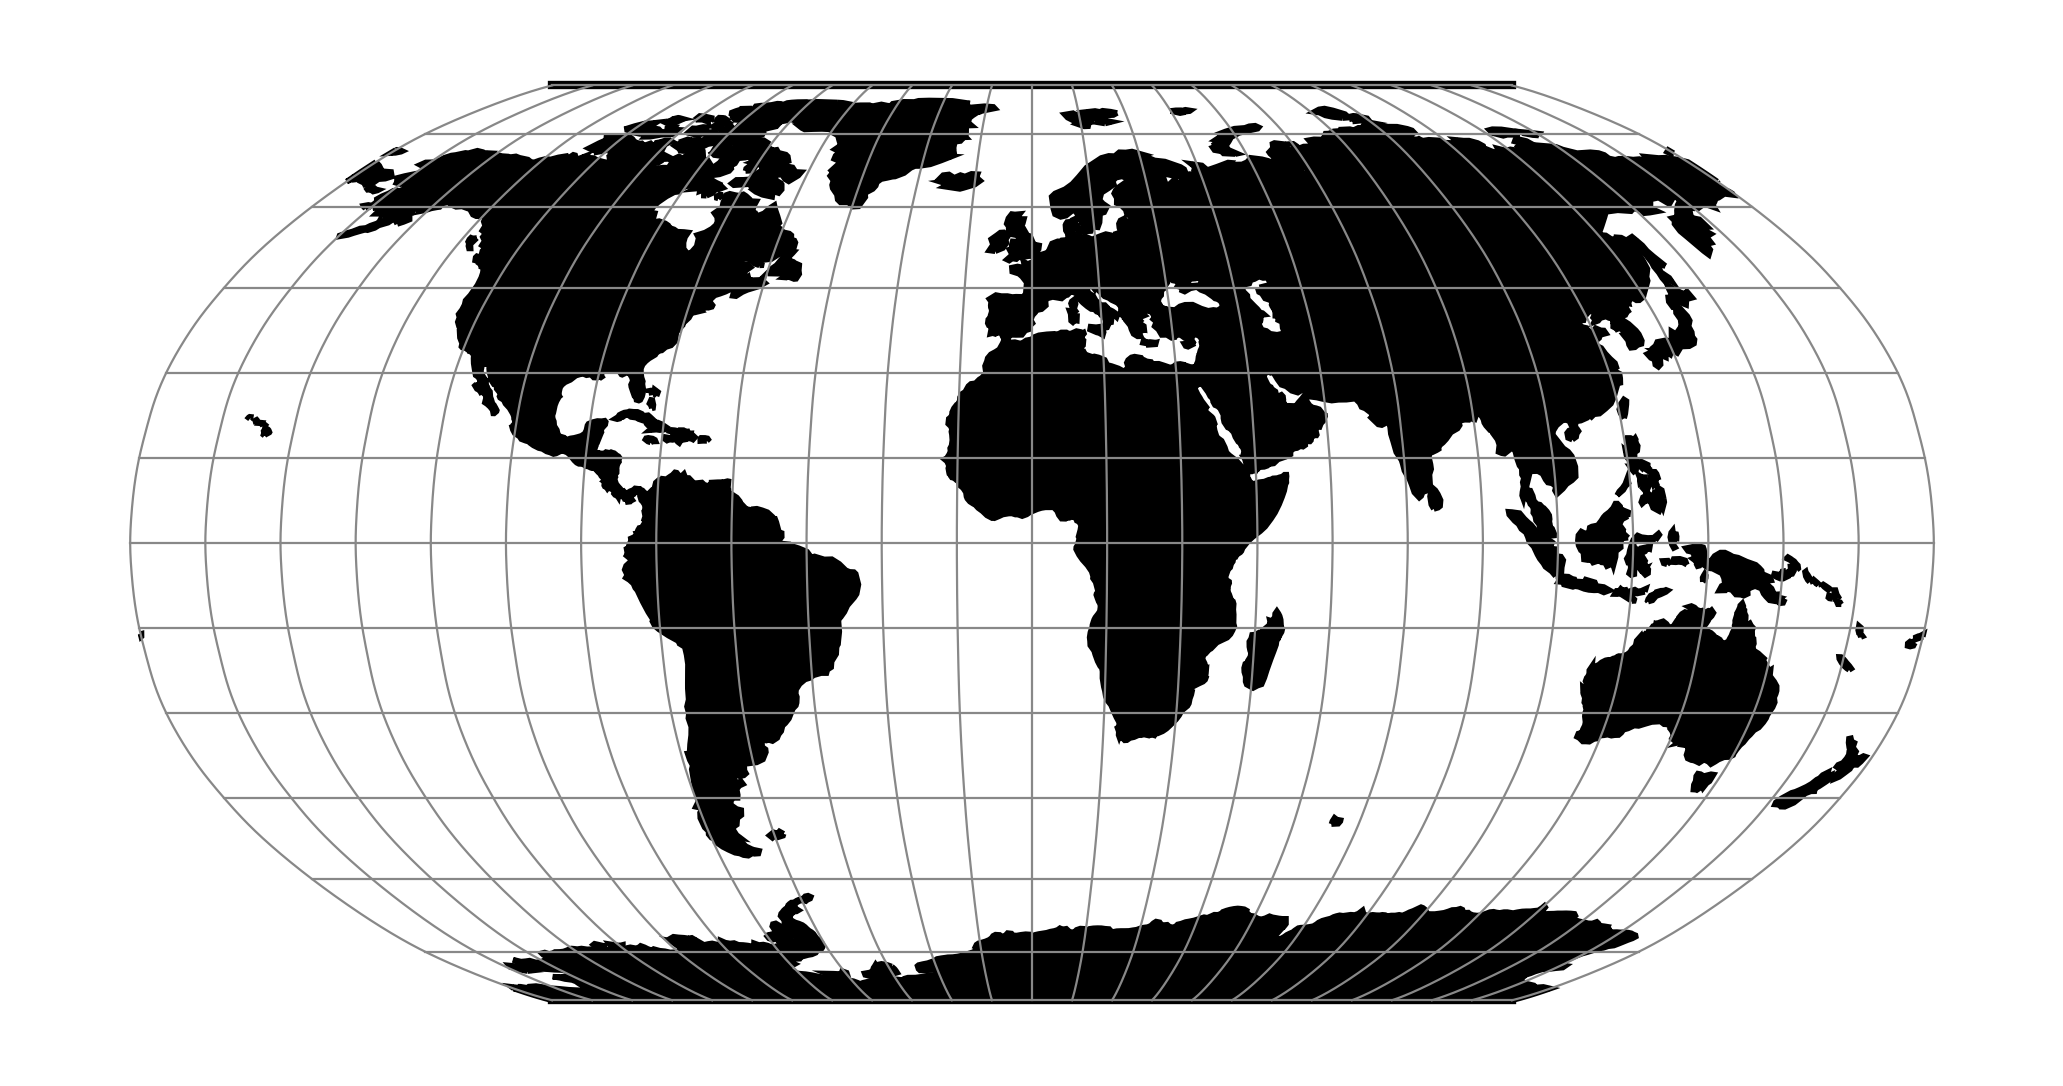
\includegraphics[width=0.9\linewidth]{figures/chapter-8/robin.png}
        \caption{Robinson (Source \cite{PROJ_SITE})}
        \label{fig:robin_proj}
    \end{minipage}\hfill
    \begin{minipage}{0.30\textwidth}
        \centering
        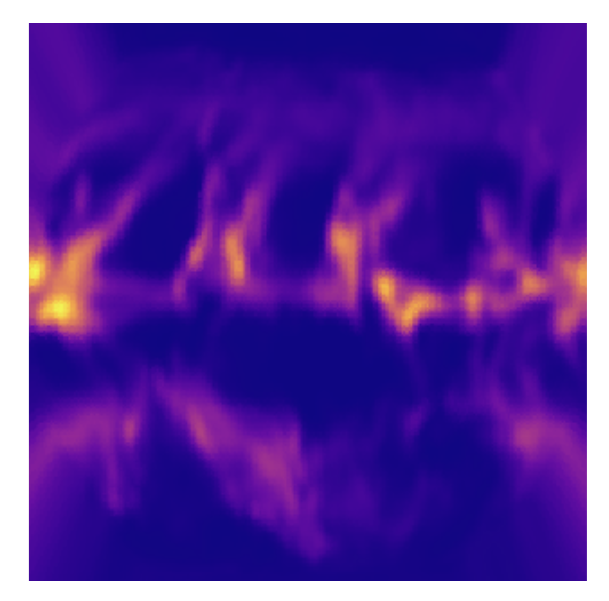
\includegraphics[width=0.9\linewidth]{figures/chapter-8/prect_robin.png}
        \caption{Precipitation raster data as Robinson projected}
        \label{fig:robin_prect_raster}
    \end{minipage}\hfill
\end{figure}
\begin{figure}[h]
    \centering
    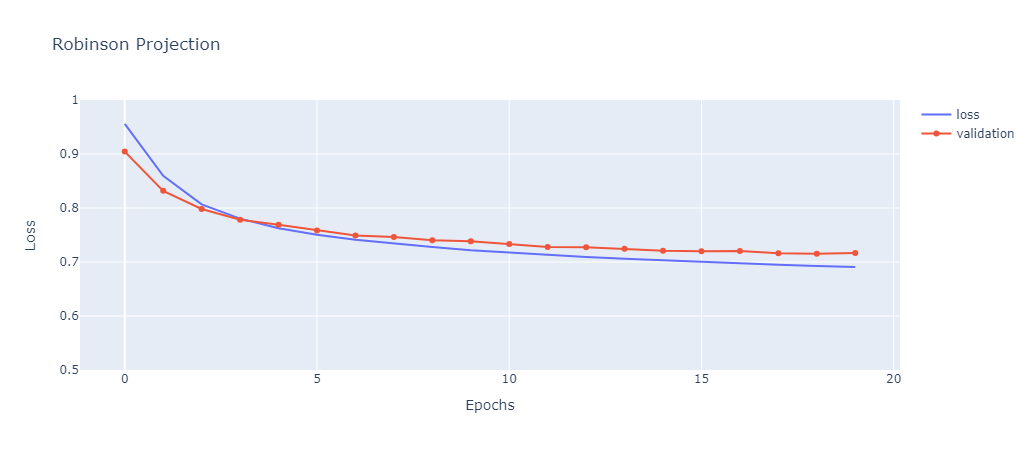
\includegraphics[width=1.0\linewidth]{figures/chapter-8/robin_loss.png}
    \caption{Robinson: Averaged training loss of models  }
    \label{fig:robin_loss}
\end{figure}
\subsubsection*{Interrupted Goode Homolosine}
\begin{figure}[h]
    \centering
    \begin{minipage}{0.30\textwidth}
        \centering
        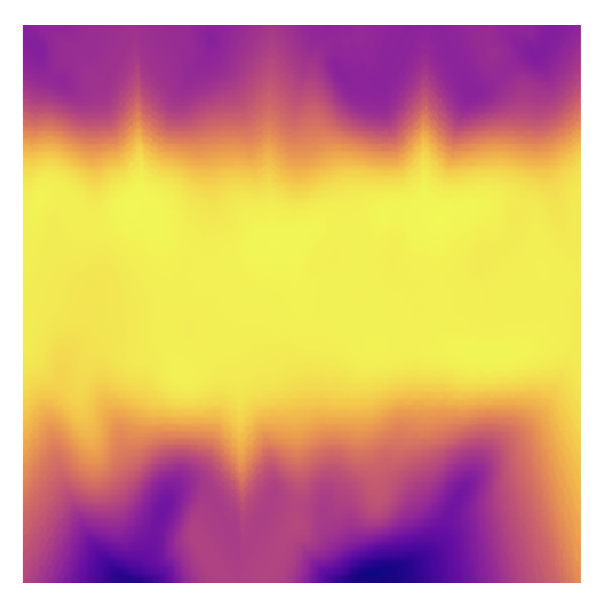
\includegraphics[width=0.9\linewidth]{figures/chapter-8/geopoth_goode.png}
        \caption{ Geopotential height raster data as Interrupted Goode Homolosine projected}
        \label{fig:ig_geopoth_raster}
    \end{minipage}\hfill
    \begin{minipage}{0.30\textwidth}
        \centering
        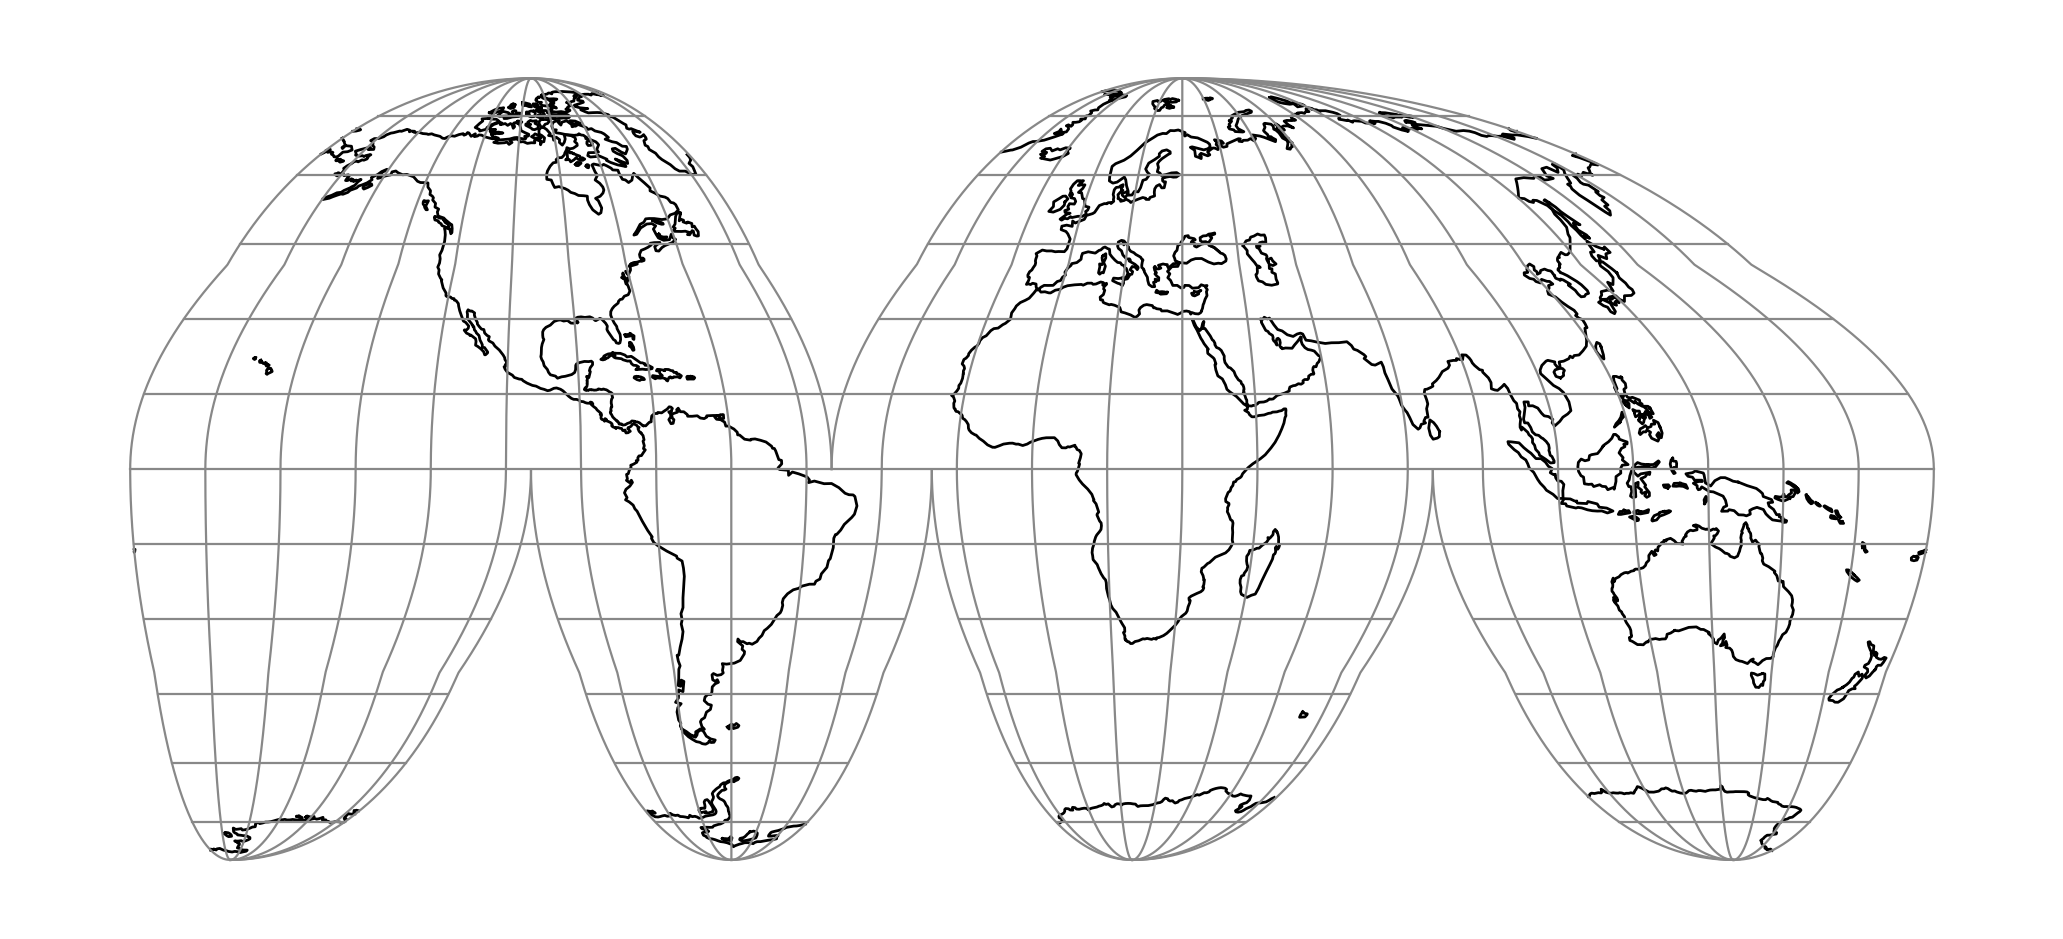
\includegraphics[width=0.9\linewidth]{figures/chapter-8/igh.png}
        \caption{Interrupted Goode Homolosine (Source \cite{PROJ_SITE})}
        \label{fig:ig_proj}
    \end{minipage}\hfill
    \begin{minipage}{0.30\textwidth}
        \centering
        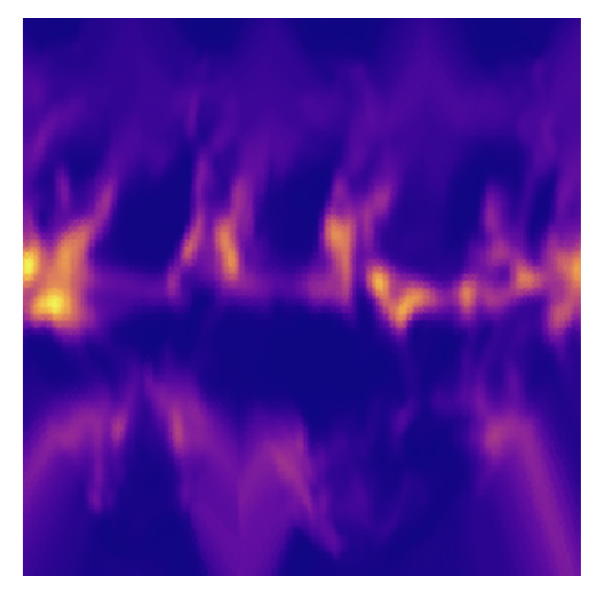
\includegraphics[width=0.9\linewidth]{figures/chapter-8/prect_goode.png}
        \caption{Precipitation raster data as Interrupted Goode Homolosine projected}
        \label{fig:ig_prect_raster}
    \end{minipage}\hfill
\end{figure}

\begin{figure}[h]
    \centering
    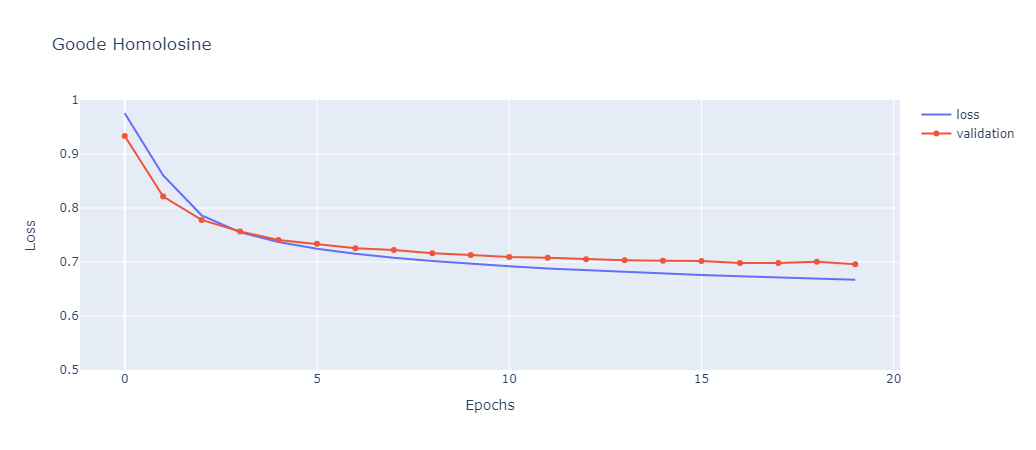
\includegraphics[width=1.0\linewidth]{figures/chapter-8/goode_loss.png}
    \caption{Interrupted Goode Homolosine: Averaged training loss of models  }
    \label{fig:goode_loss}
\end{figure}
\newpage
\subsubsection*{Sinusoidal Sanson Flamsteed}
\begin{figure}[h]
    \centering
    \begin{minipage}{0.30\textwidth}
        \centering
        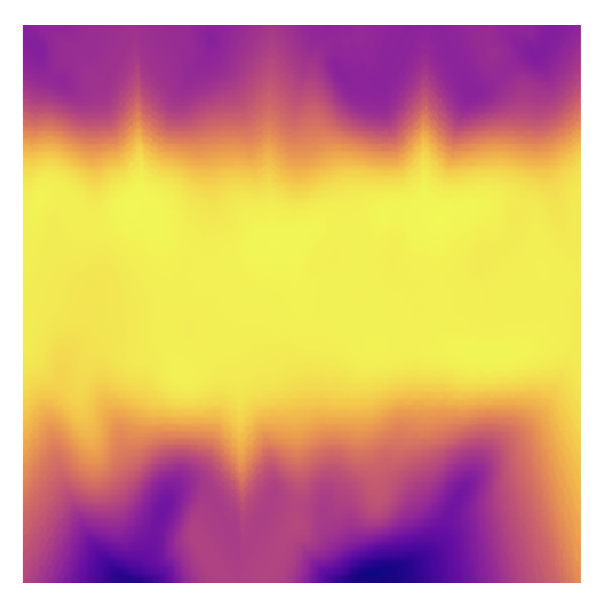
\includegraphics[width=0.9\linewidth]{figures/chapter-8/geopoth_goode.png}
        \caption{ Geopotential height raster data as Sinusoidal Sanson Flamsteed projected}
        \label{fig:ig_geopoth_raster}
    \end{minipage}\hfill
    \begin{minipage}{0.30\textwidth}
        \centering
        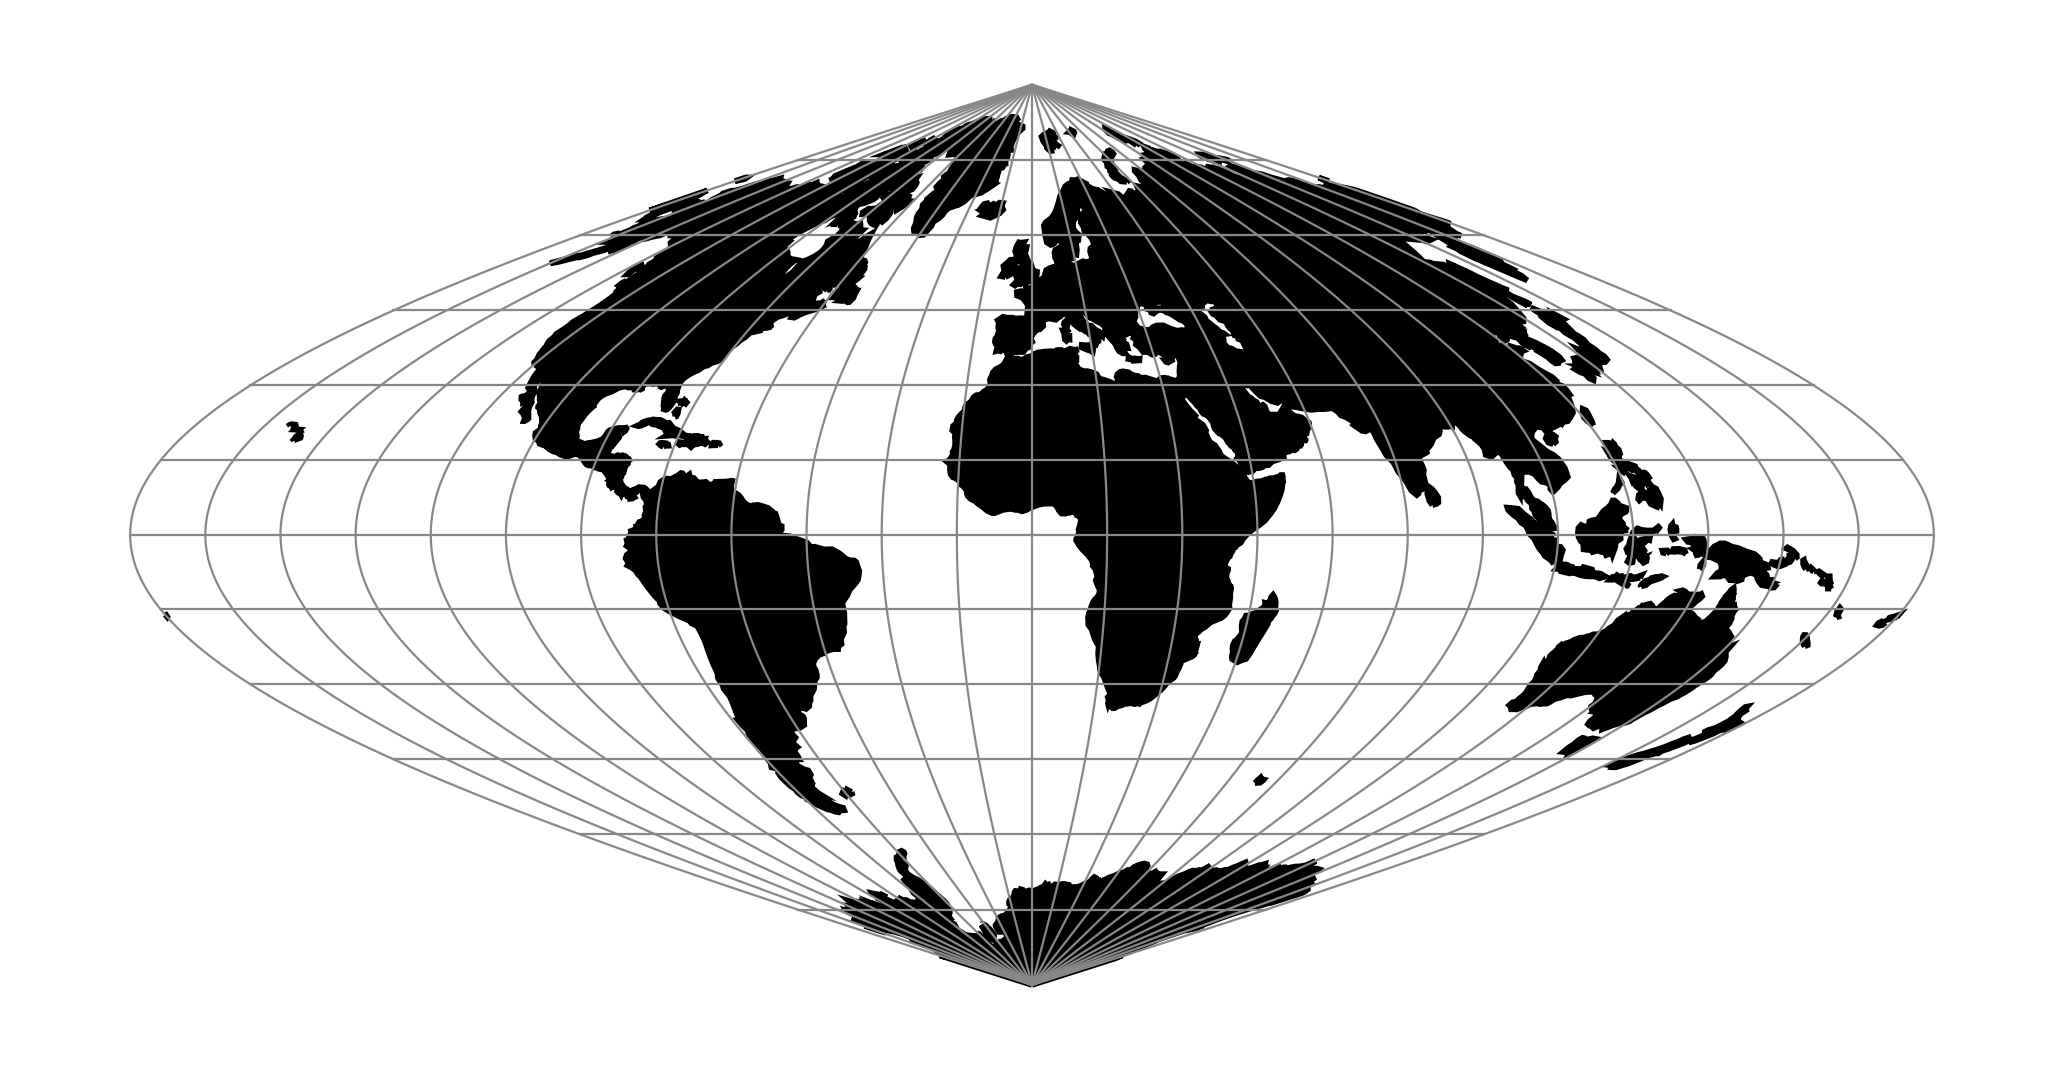
\includegraphics[width=0.9\linewidth]{figures/chapter-8/sinu.png}
        \caption{Sinusoidal Sanson Flamsteed (Source \cite{PROJ_SITE})}
        \label{fig:ig_proj}
    \end{minipage}\hfill
    \begin{minipage}{0.30\textwidth}
        \centering
        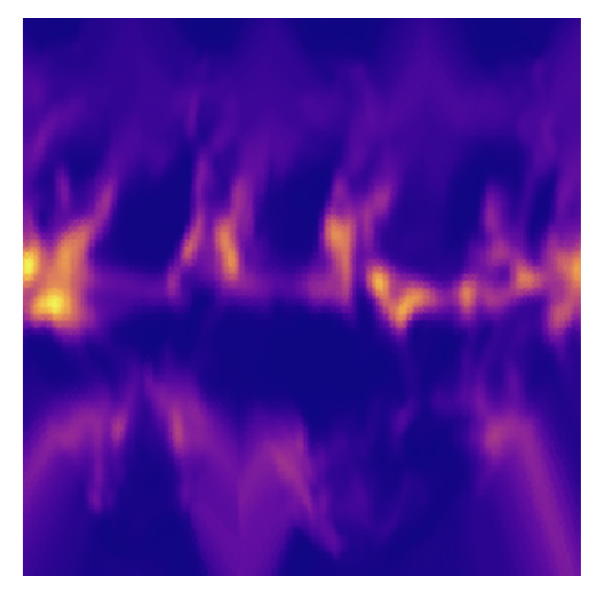
\includegraphics[width=0.9\linewidth]{figures/chapter-8/prect_goode.png}
        \caption{Precipitation raster data as Sinusoidal Sanson Flamsteed projected}
        \label{fig:ig_prect_raster}
    \end{minipage}\hfill
\end{figure}


\begin{figure}[h]
    \centering
    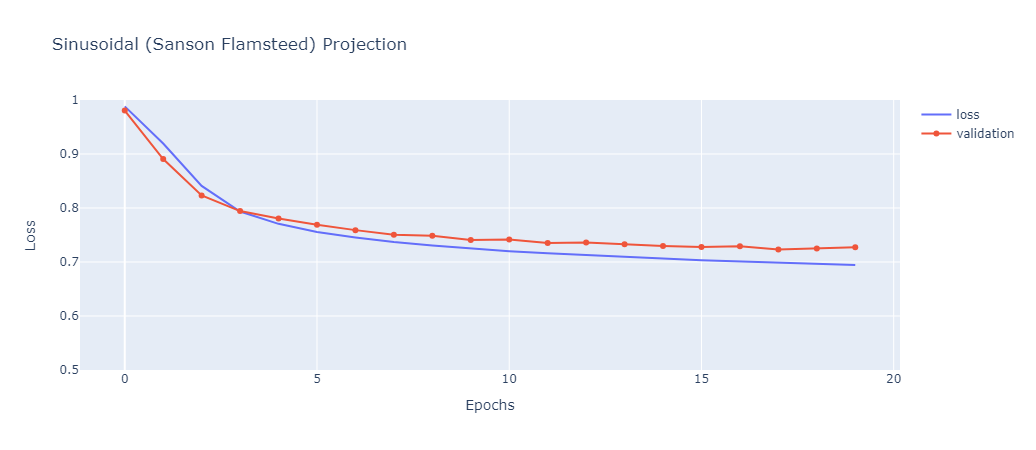
\includegraphics[width=1.0\linewidth]{figures/chapter-8/sinu_loss.png}
    \caption{Sinusoidal Sanson Flamsteed: Averaged training loss of models  }
    \label{fig:sinu_loss}
\end{figure}
\subsubsection*{Loximuthal}
\subsection{Results}

\newpage
\section{Conic Projections}
\subsubsection*{Lambert Equal Area Conic}
\begin{figure}[h]
    \centering
    \begin{minipage}{0.30\textwidth}
        \centering
        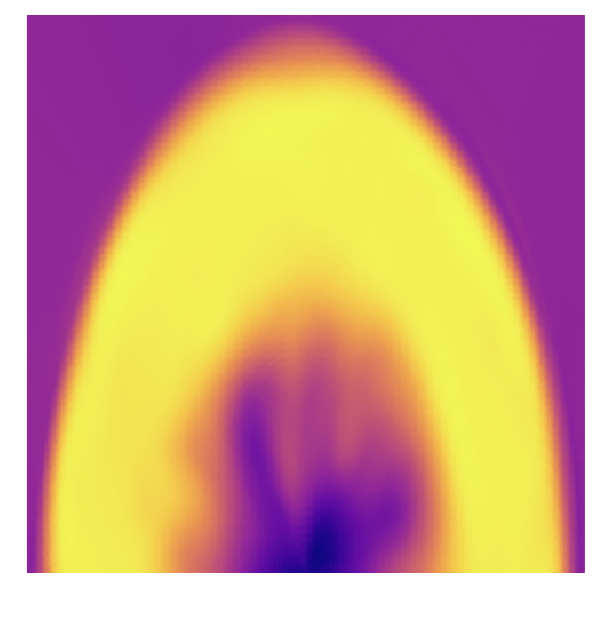
\includegraphics[width=0.9\linewidth]{figures/chapter-8/geopoth_leac.png}
        \caption{ Geopotential height raster data as Lambert Equal Area Conic projected}
        \label{fig:leac_geopoth_raster}
    \end{minipage}\hfill
    \begin{minipage}{0.30\textwidth}
        \centering
        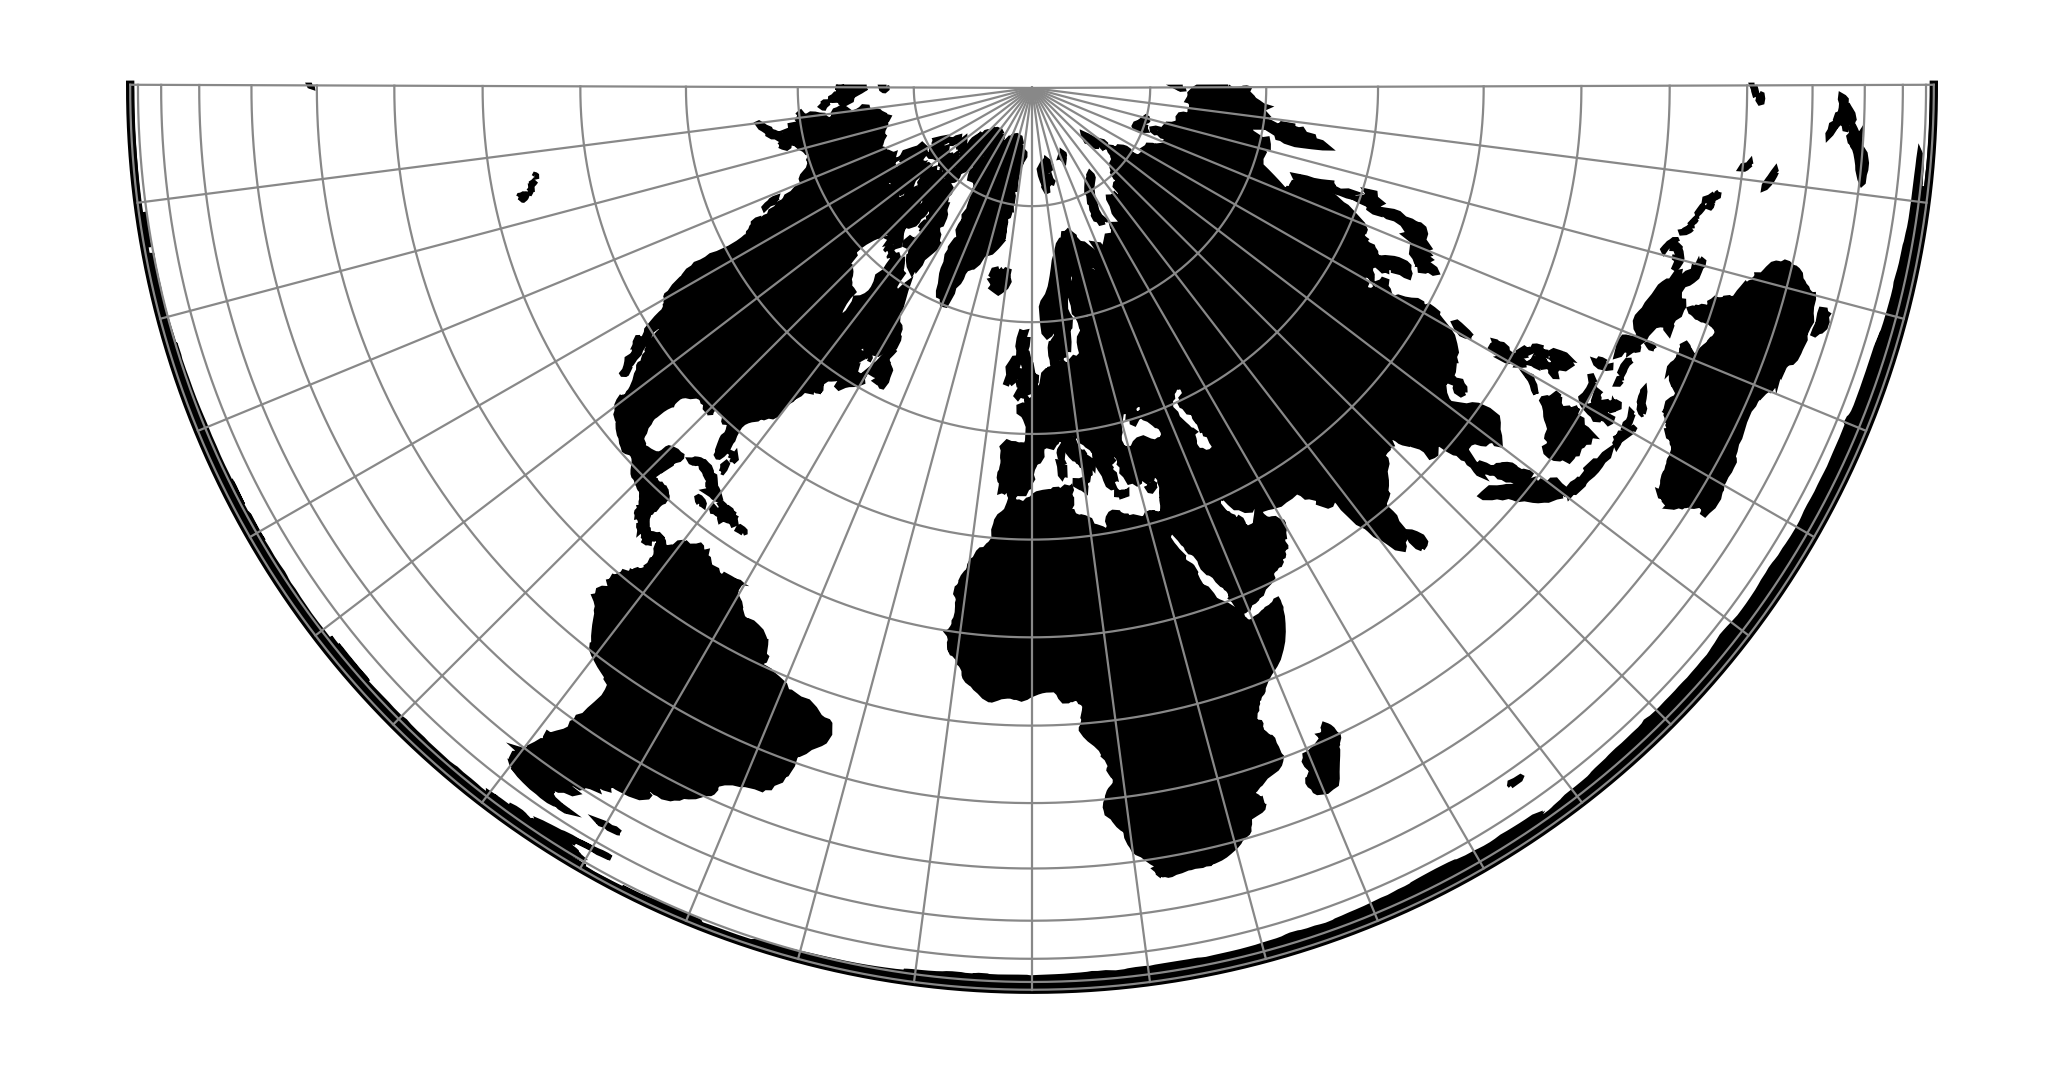
\includegraphics[width=0.9\linewidth]{figures/chapter-8/leac.png}
        \caption{Lambert Equal Area Conic (Source \cite{PROJ_SITE})}
        \label{fig:leac_proj}
    \end{minipage}\hfill
    \begin{minipage}{0.30\textwidth}
        \centering
        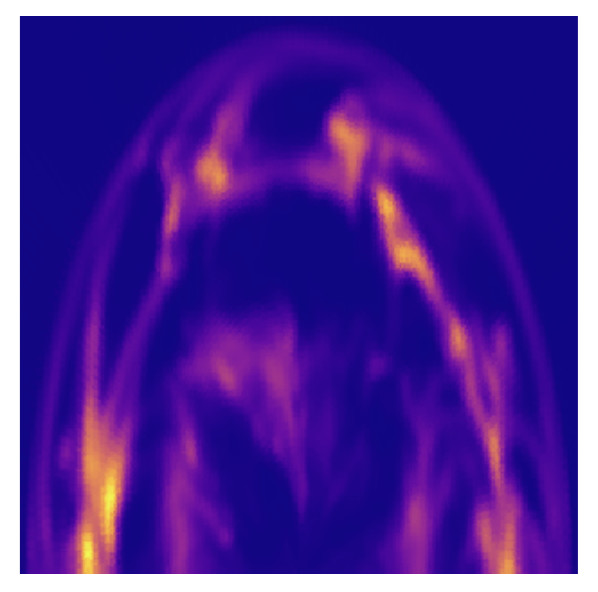
\includegraphics[width=0.9\linewidth]{figures/chapter-8/prect_leac.png}
        \caption{Precipitation raster data as Lambert Equal Area Conic projected}
        \label{fig:leac_prect_raster}
    \end{minipage}\hfill
\end{figure}
\subsubsection*{Albers Equal Area}
\begin{figure}[h]
    \centering
    \begin{minipage}{0.30\textwidth}
        \centering
        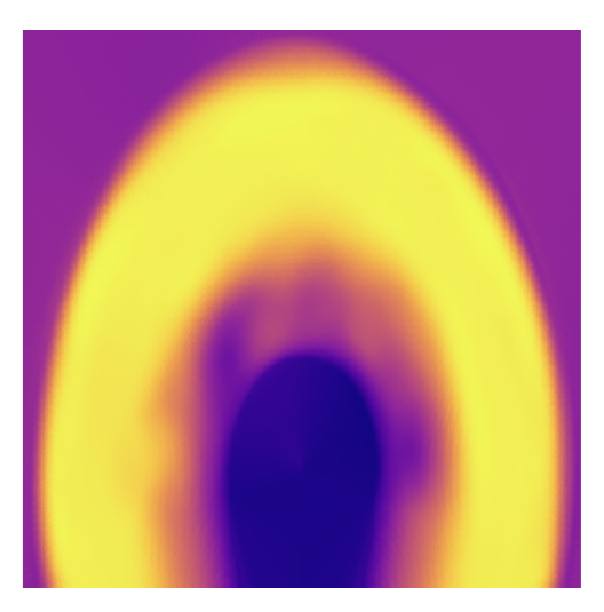
\includegraphics[width=0.9\linewidth]{figures/chapter-8/geopoth_aea.png}
        \caption{ Geopotential height raster data as Albers Equal Area projected}
        \label{fig:aea_geopoth_raster}
    \end{minipage}\hfill
    \begin{minipage}{0.30\textwidth}
        \centering
        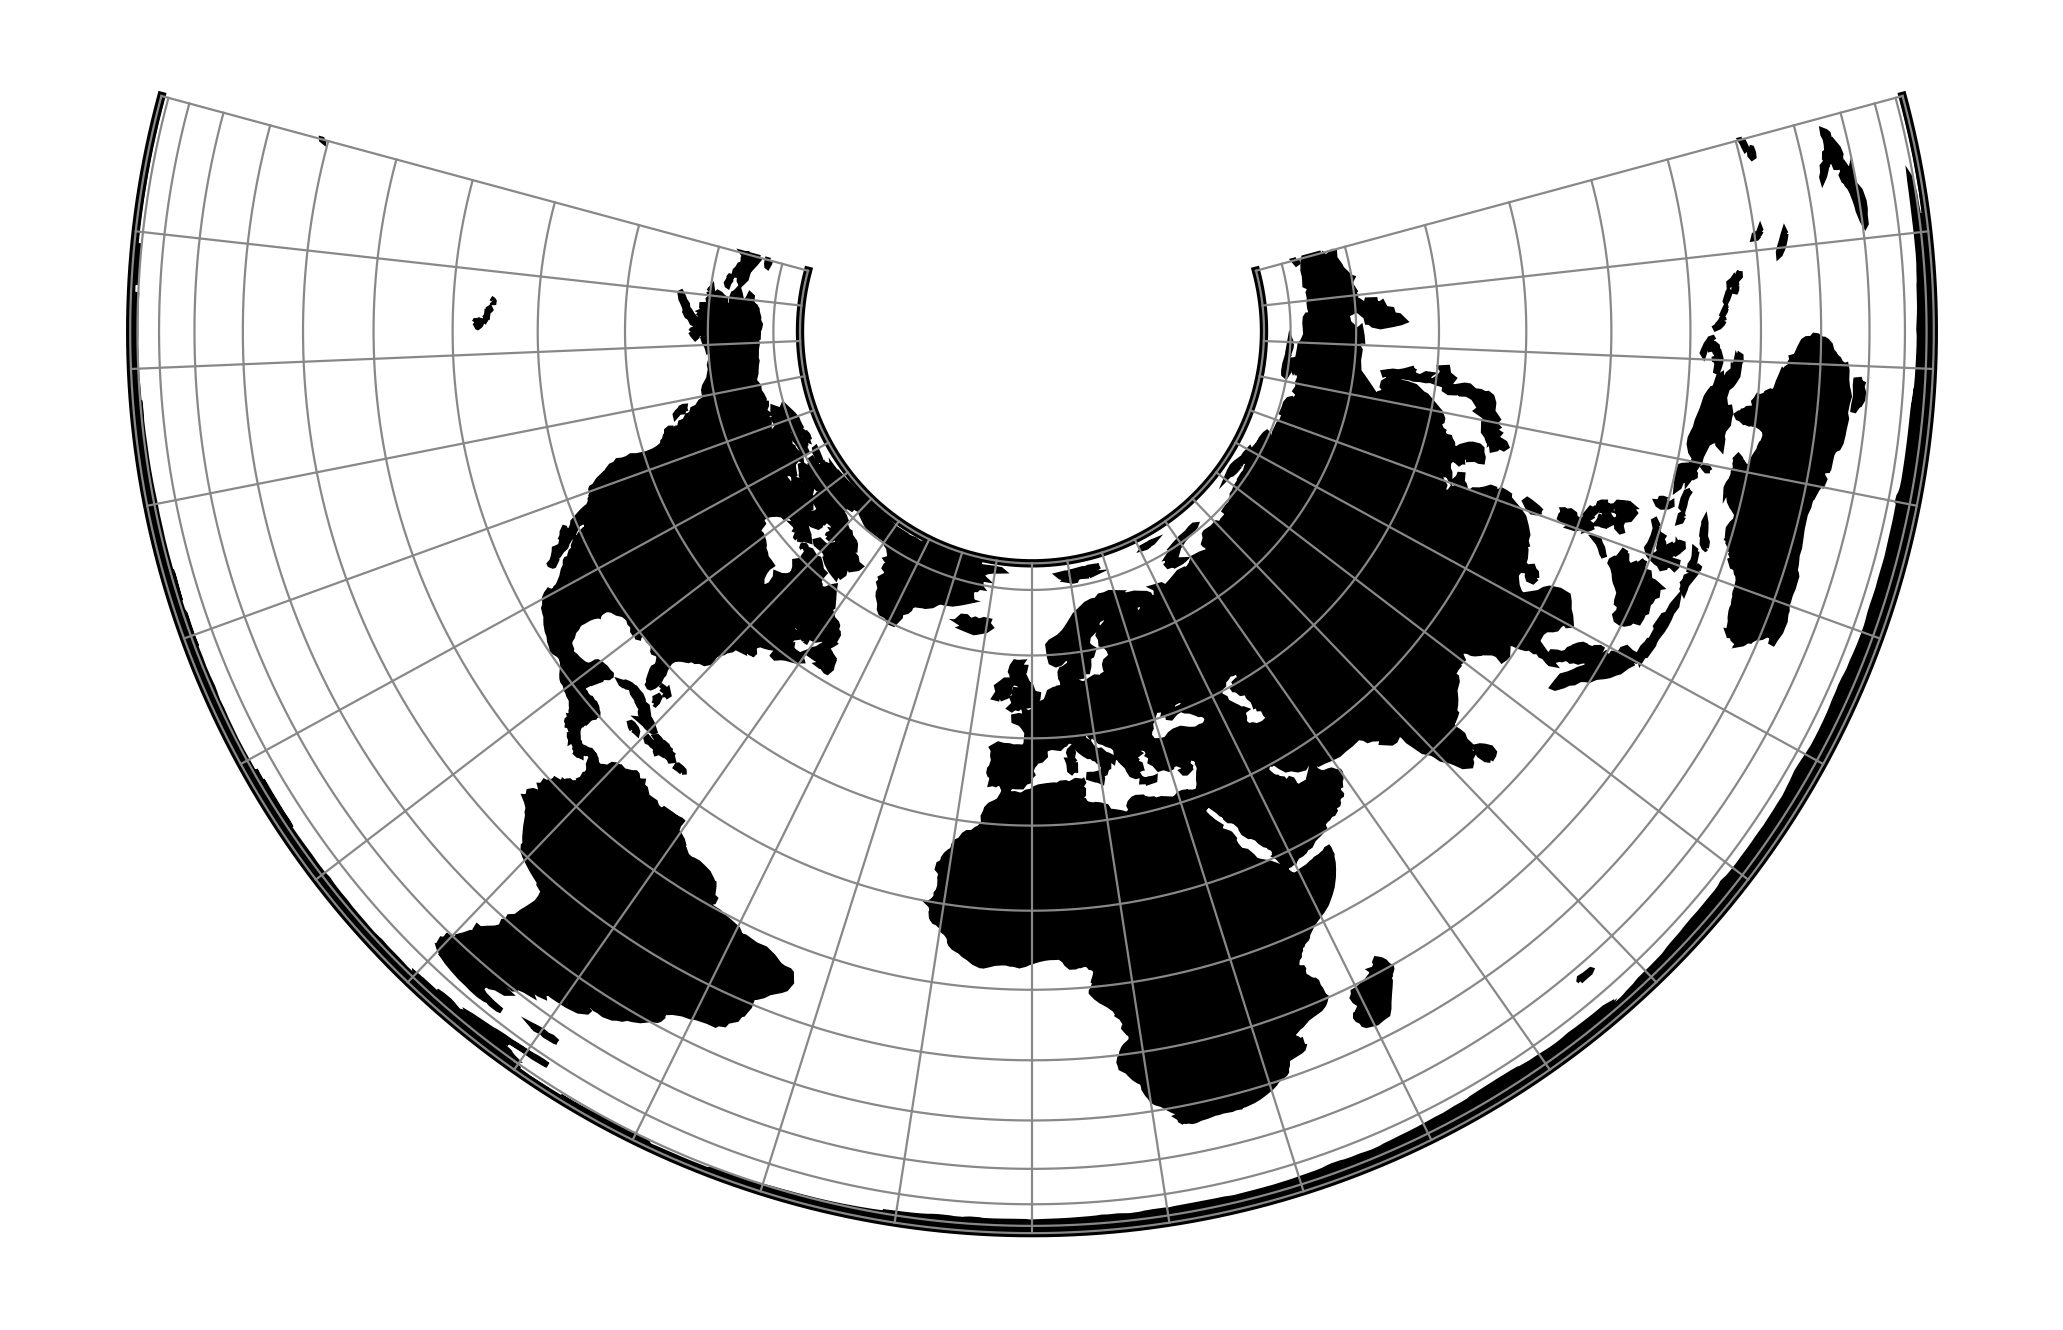
\includegraphics[width=0.9\linewidth]{figures/chapter-8/aea.png}
        \caption{Albers Equal Area (Source \cite{PROJ_SITE})}
        \label{fig:aea_proj}
    \end{minipage}\hfill
    \begin{minipage}{0.30\textwidth}
        \centering
        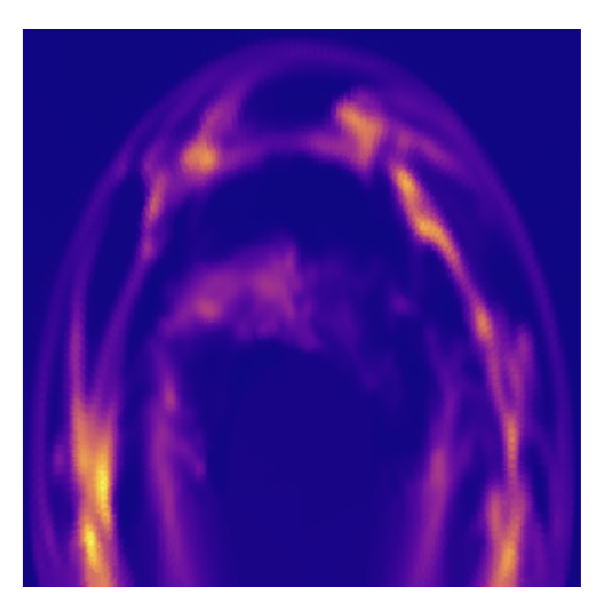
\includegraphics[width=0.9\linewidth]{figures/chapter-8/prect_aea.png}
        \caption{Precipitation raster data as Albers Equal Area projected}
        \label{fig:aea_prect_raster}
    \end{minipage}\hfill
\end{figure}
\newpage
\subsubsection*{Vitkovsky I}
\begin{figure}[h]
    \centering
    \begin{minipage}{0.30\textwidth}
        \centering
        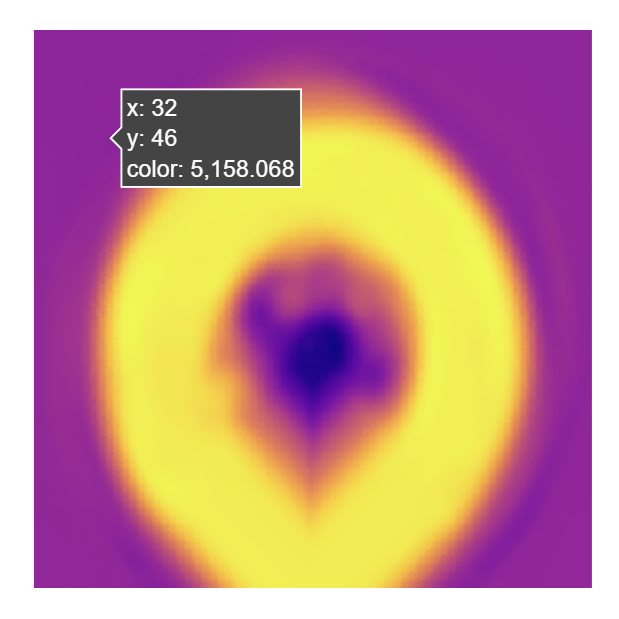
\includegraphics[width=0.9\linewidth]{figures/chapter-8/geopoth_vitk.png}
        \caption{ Geopotential height raster data as Vitkovsky I projected}
        \label{fig:vitk_geopoth_raster}
    \end{minipage}\hfill
    \begin{minipage}{0.30\textwidth}
        \centering
        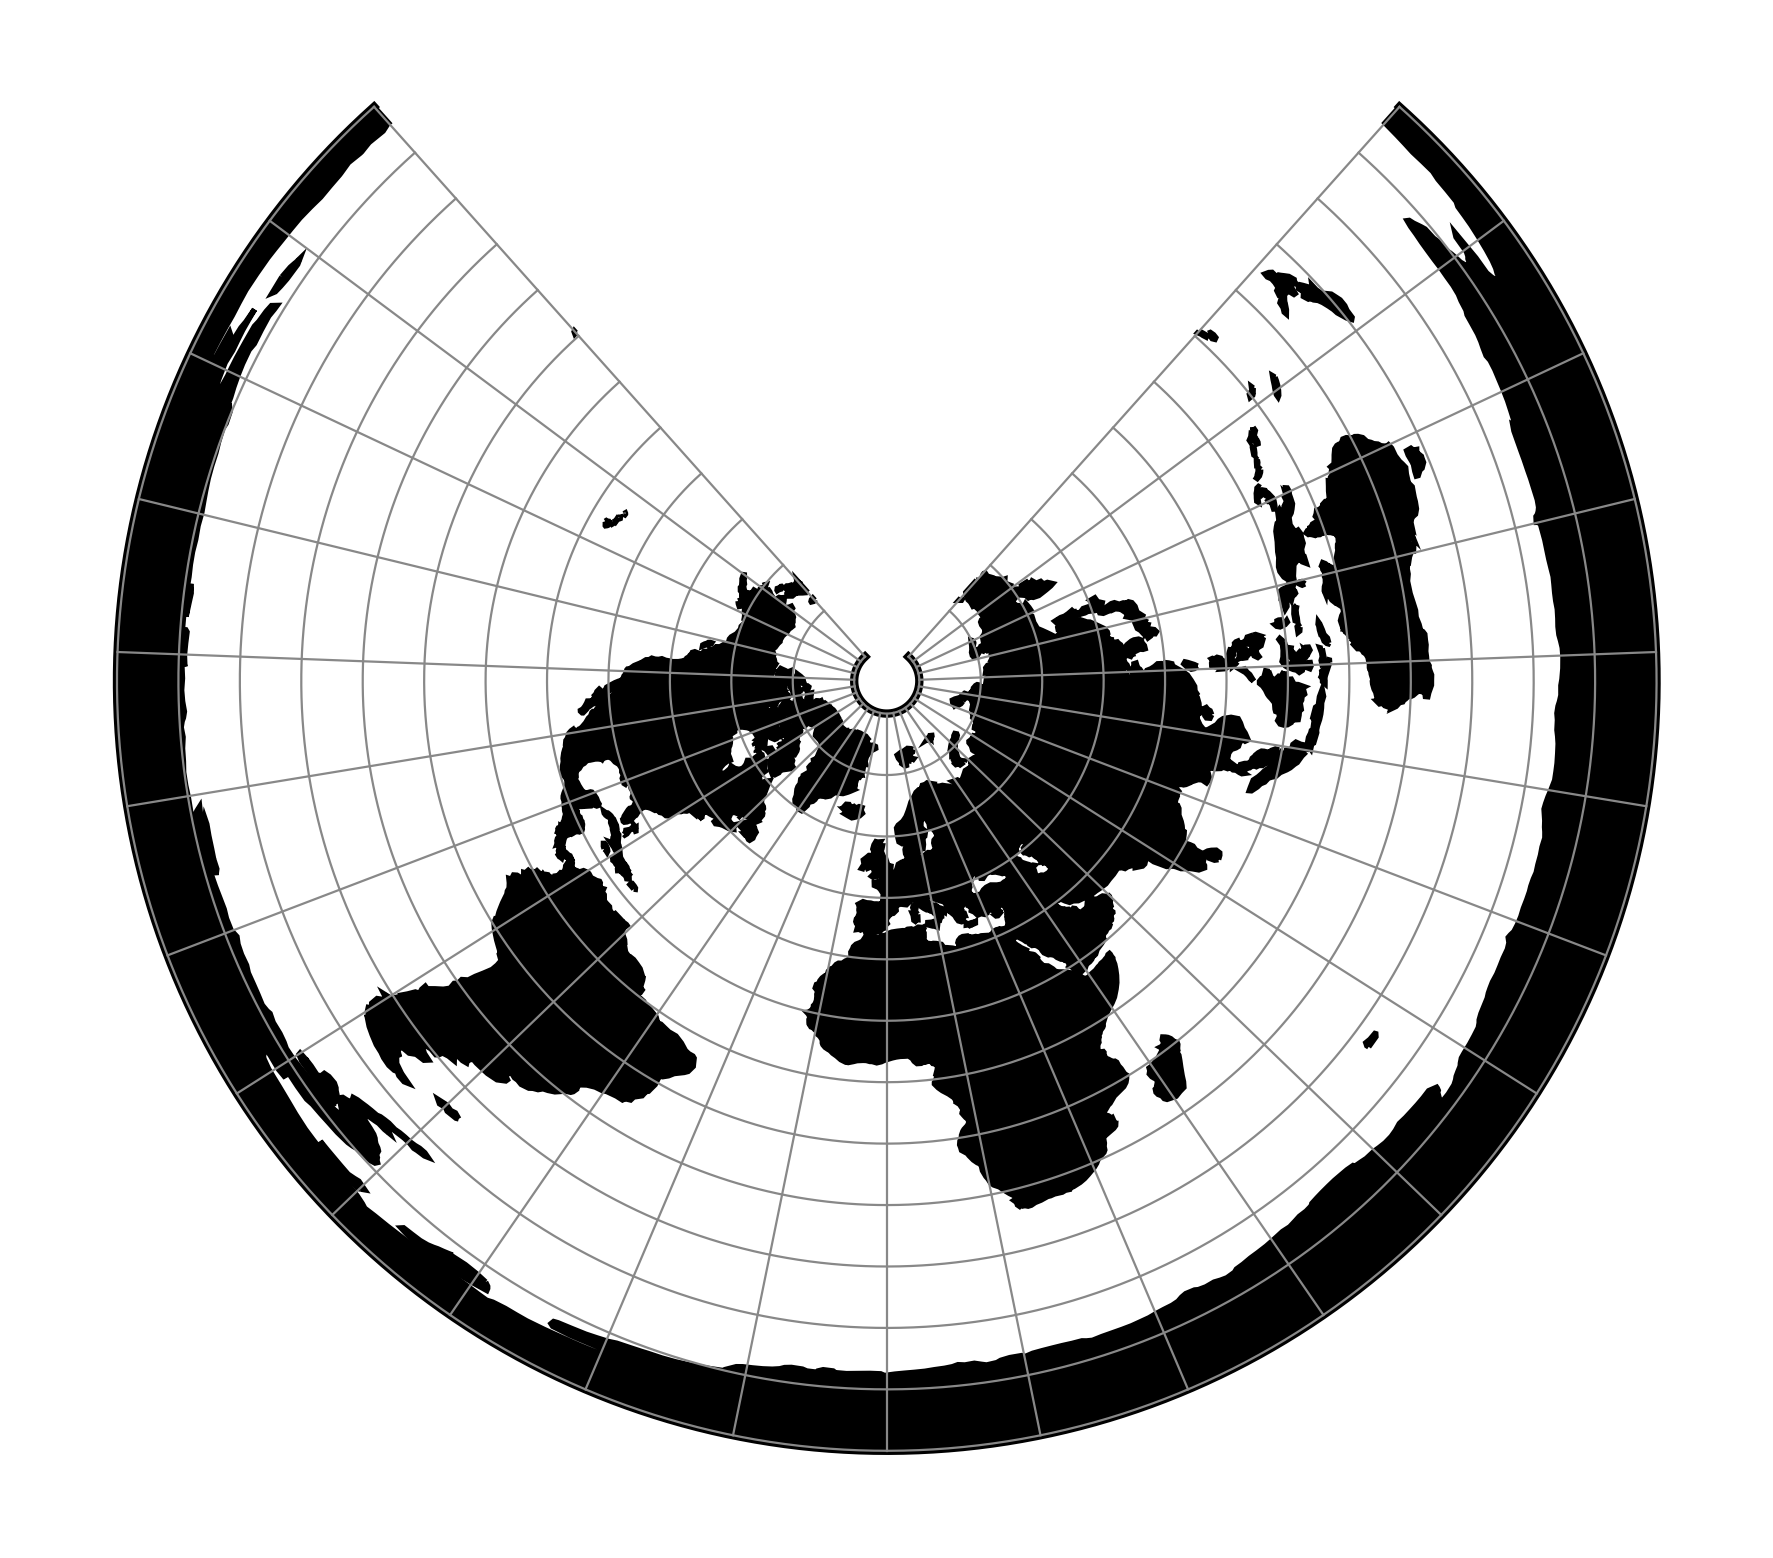
\includegraphics[width=0.9\linewidth]{figures/chapter-8/vitk1.png}
        \caption{Vitkovsky I (Source \cite{PROJ_SITE})}
        \label{fig:vitk_proj}
    \end{minipage}\hfill
    \begin{minipage}{0.30\textwidth}
        \centering
        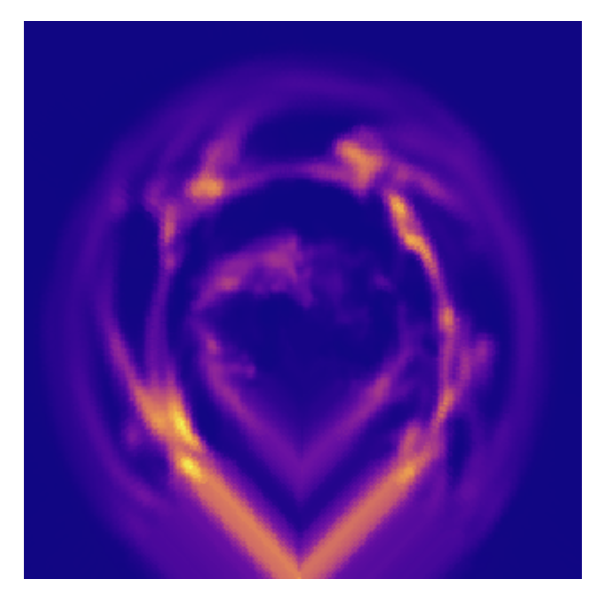
\includegraphics[width=0.9\linewidth]{figures/chapter-8/prect_vitk.png}
        \caption{Precipitation raster data as Vitkovsky I projected}
        \label{fig:vitk_prect_raster}
    \end{minipage}\hfill
\end{figure}
\subsubsection*{Lambert Conformal Conic Alternative}
\begin{figure}[h]
    \centering
    \begin{minipage}{0.30\textwidth}
        \centering
        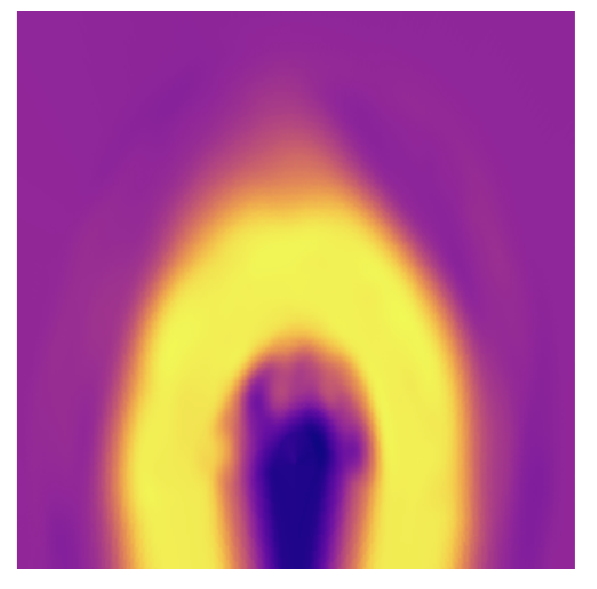
\includegraphics[width=0.9\linewidth]{figures/chapter-8/geopoth_lcca.png}
        \caption{ Geopotential height raster data as Lambert Conformal Conic Alternative projected}
        \label{fig:lcca_geopoth_raster}
    \end{minipage}\hfill
    \begin{minipage}{0.30\textwidth}
        \centering
        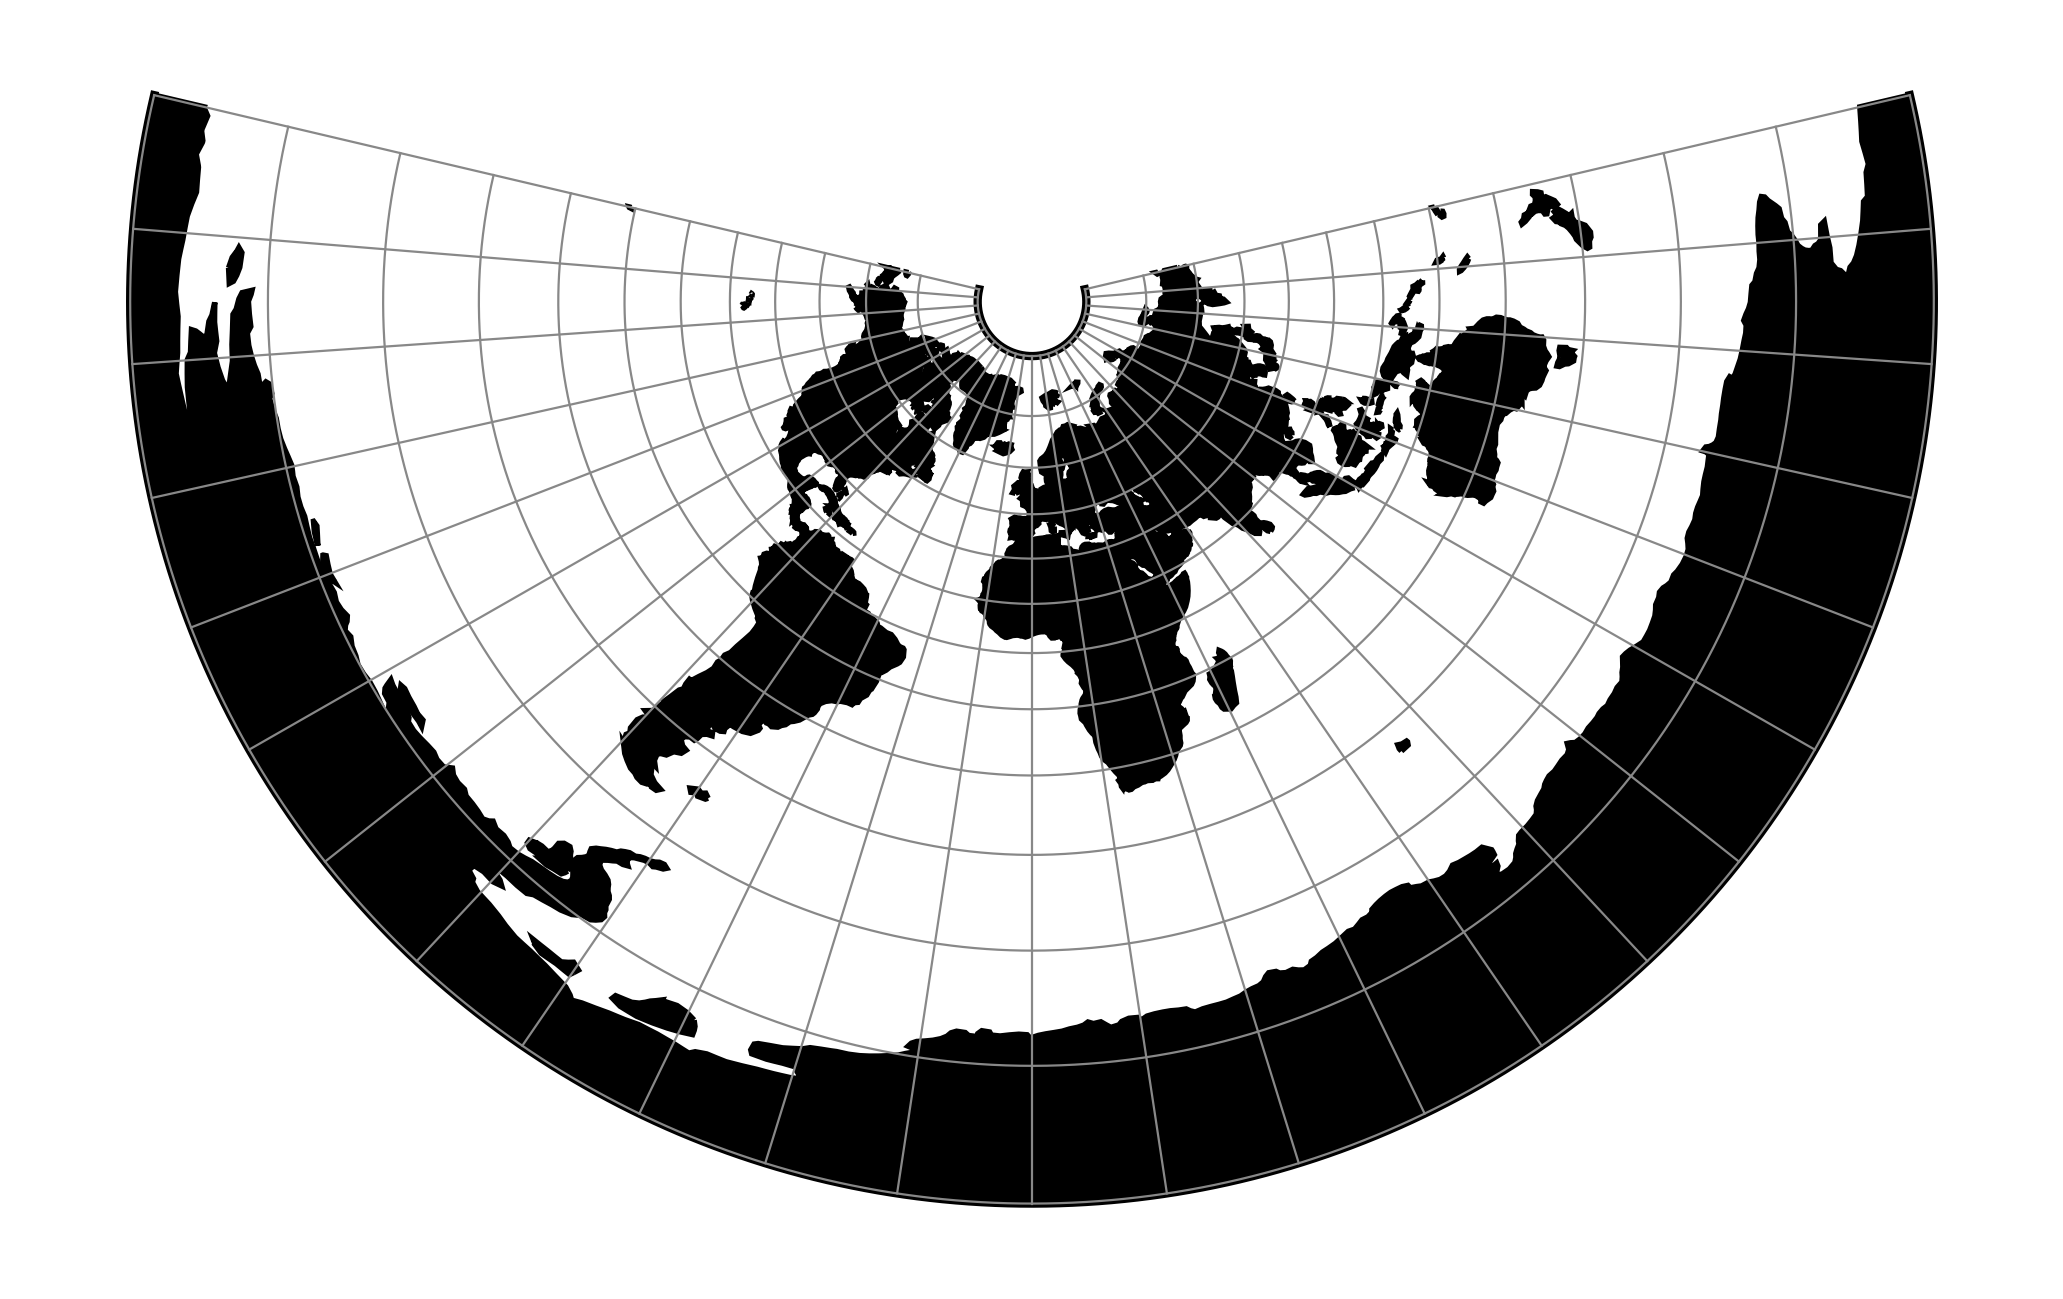
\includegraphics[width=0.9\linewidth]{figures/chapter-8/lcca.png}
        \caption{Lambert Conformal Conic Alternative (Source \cite{PROJ_SITE})}
        \label{fig:lcca_proj}
    \end{minipage}\hfill
    \begin{minipage}{0.30\textwidth}
        \centering
        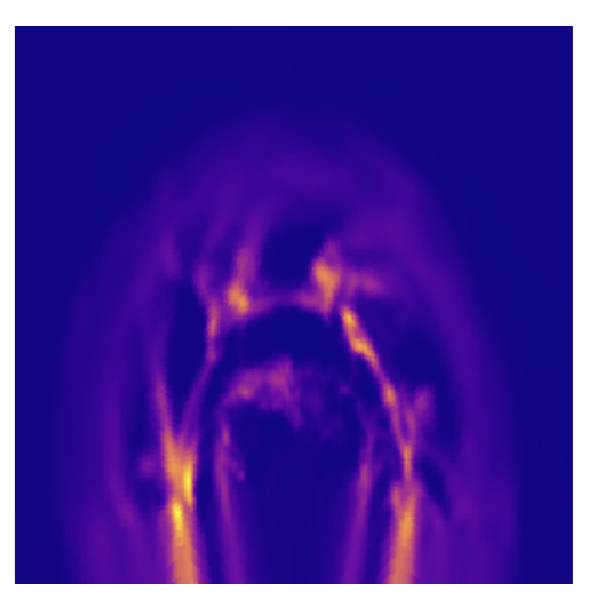
\includegraphics[width=0.9\linewidth]{figures/chapter-8/prect_lcca.png}
        \caption{Precipitation raster data as Lambert Conformal Conic Alternative projected}
        \label{fig:lcca_prect_raster}
    \end{minipage}\hfill
\end{figure}

\subsection{Results}



\newpage
\section{Planar Projections}

\subsubsection*{Lambert Azimuthal Equal Area}
\begin{figure}[h]
    \centering
    \begin{minipage}{0.30\textwidth}
        \centering
        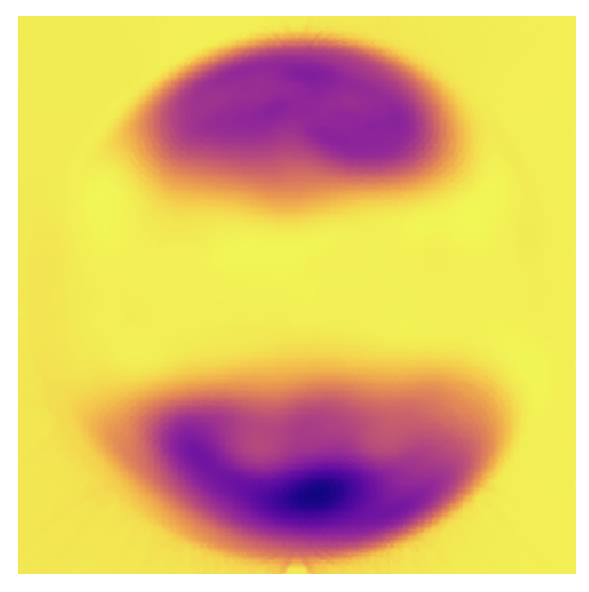
\includegraphics[width=0.9\linewidth]{figures/chapter-8/geopoth_laea.png}
        \caption{ Geopotential height raster data as Lambert Azimuthal Equal Area projected}
        \label{fig:laea_geopoth_raster}
    \end{minipage}\hfill
    \begin{minipage}{0.30\textwidth}
        \centering
        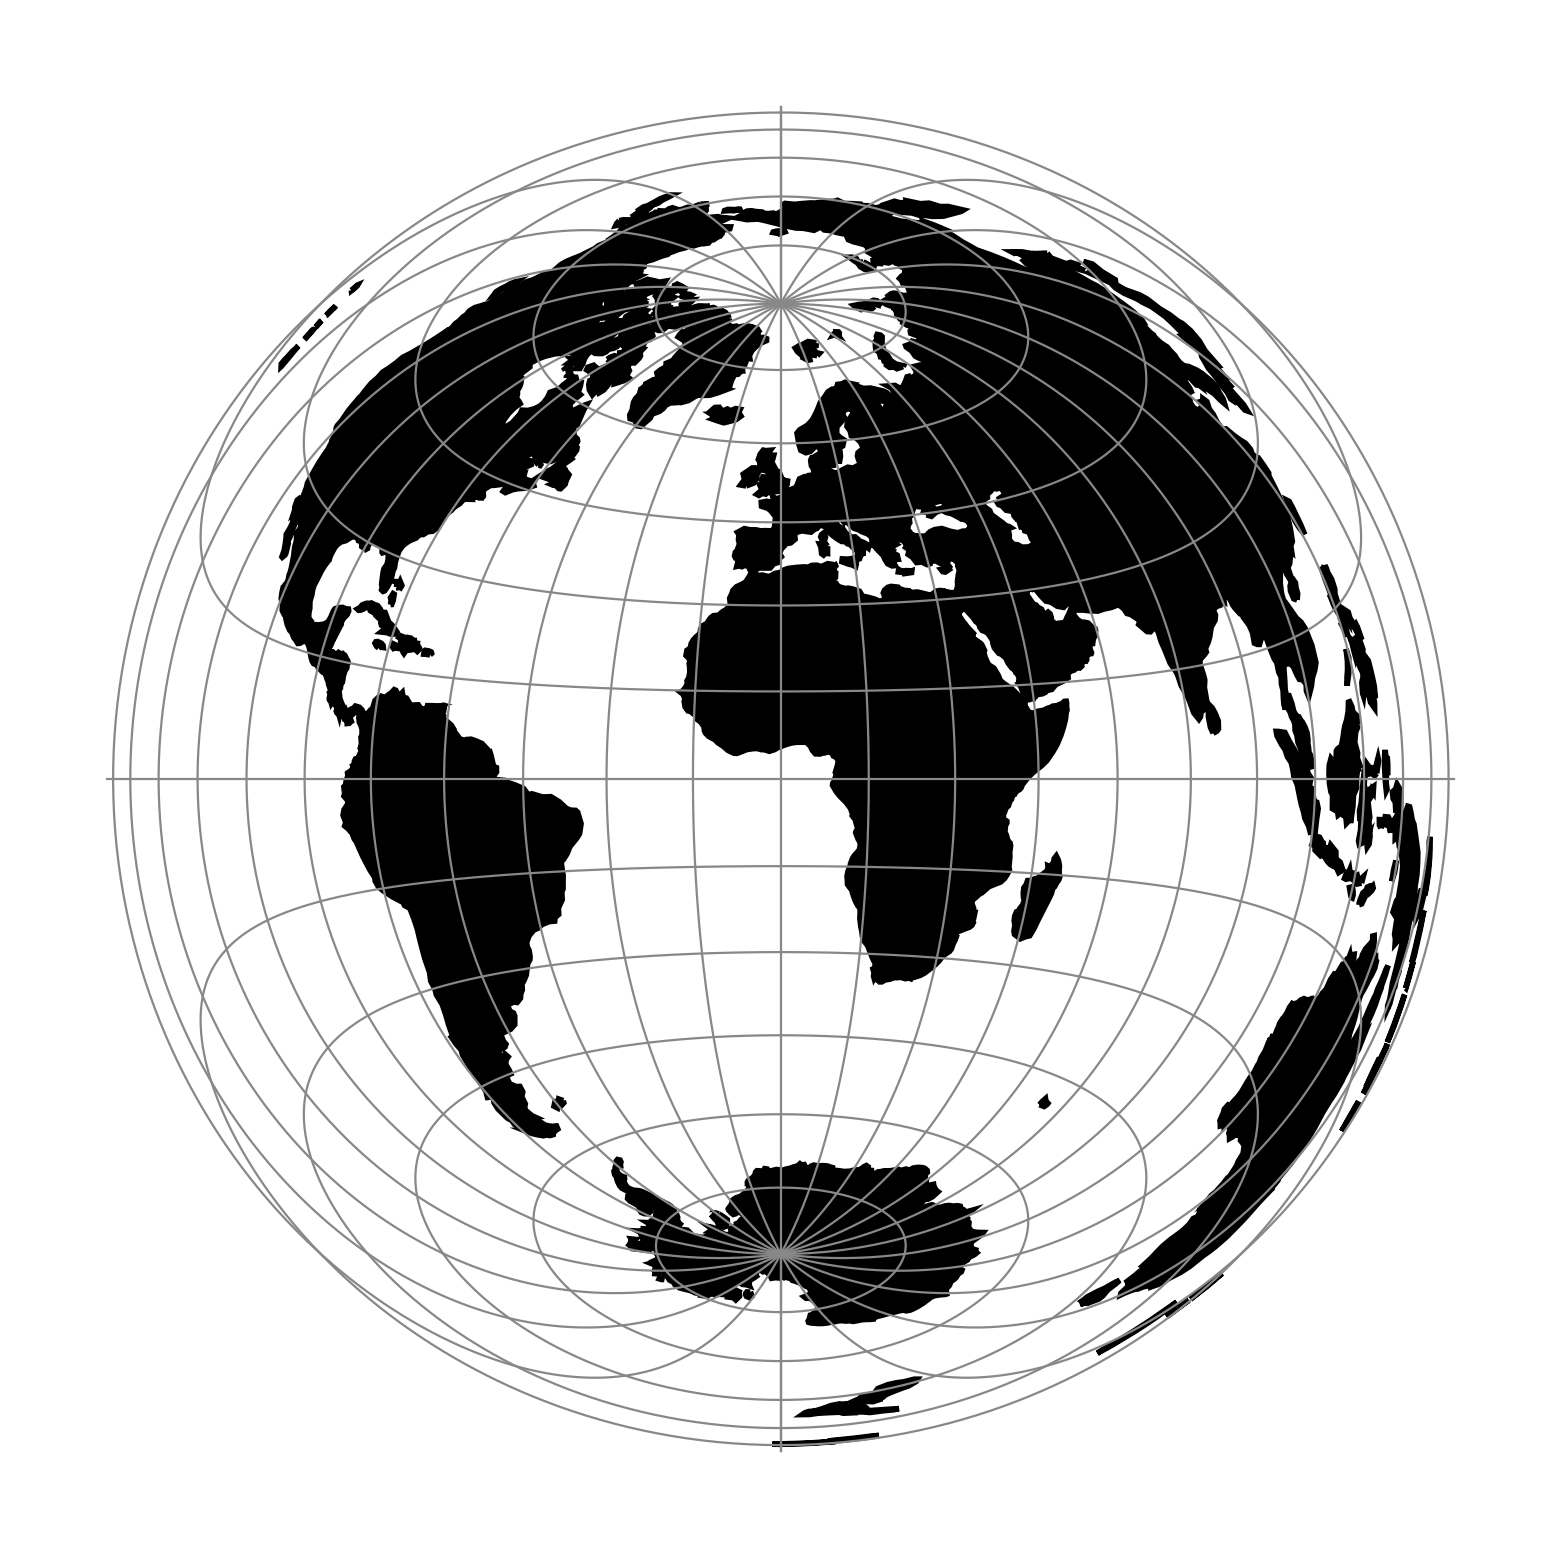
\includegraphics[width=0.9\linewidth]{figures/chapter-8/laea.png}
        \caption{Lambert Azimuthal Equal Area (Source \cite{PROJ_SITE})}
        \label{fig:laea_proj}
    \end{minipage}\hfill
    \begin{minipage}{0.30\textwidth}
        \centering
        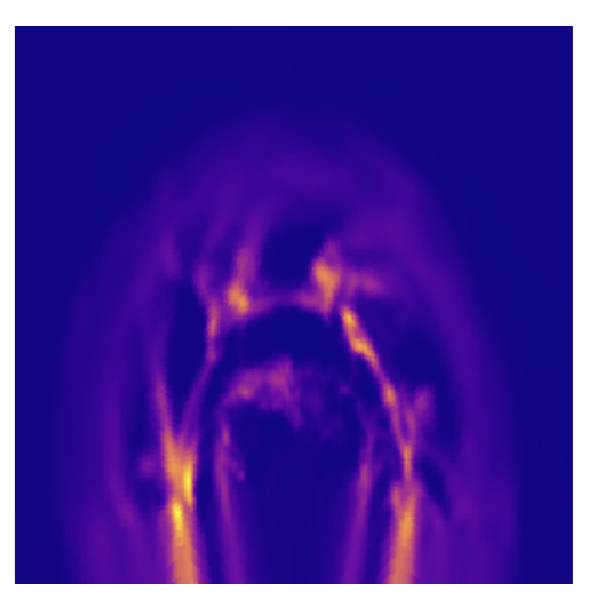
\includegraphics[width=0.9\linewidth]{figures/chapter-8/prect_lcca.png}
        \caption{Precipitation raster data as Lambert Azimuthal Equal Area projected}
        \label{fig:laea_prect_raster}
    \end{minipage}\hfill
\end{figure}

\subsubsection*{Wagner VII}
\begin{figure}[h]
    \centering
    \begin{minipage}{0.30\textwidth}
        \centering
        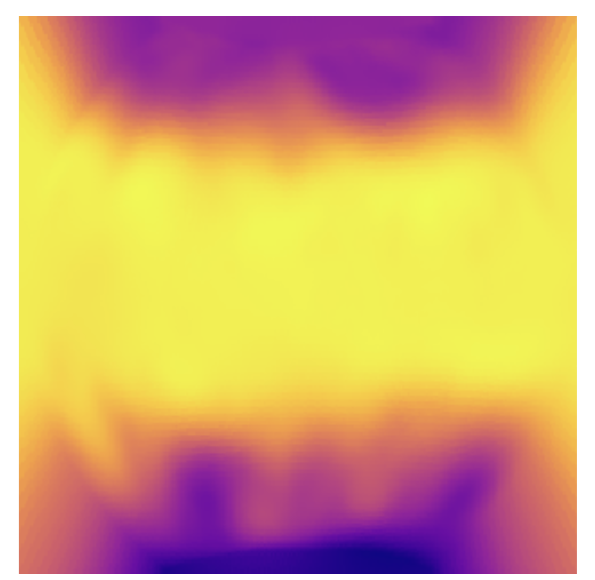
\includegraphics[width=0.9\linewidth]{figures/chapter-8/geopoth_wag.png}
        \caption{ Geopotential height raster data as Wagner VII projected}
        \label{fig:wag_geopoth_raster}
    \end{minipage}\hfill
    \begin{minipage}{0.30\textwidth}
        \centering
        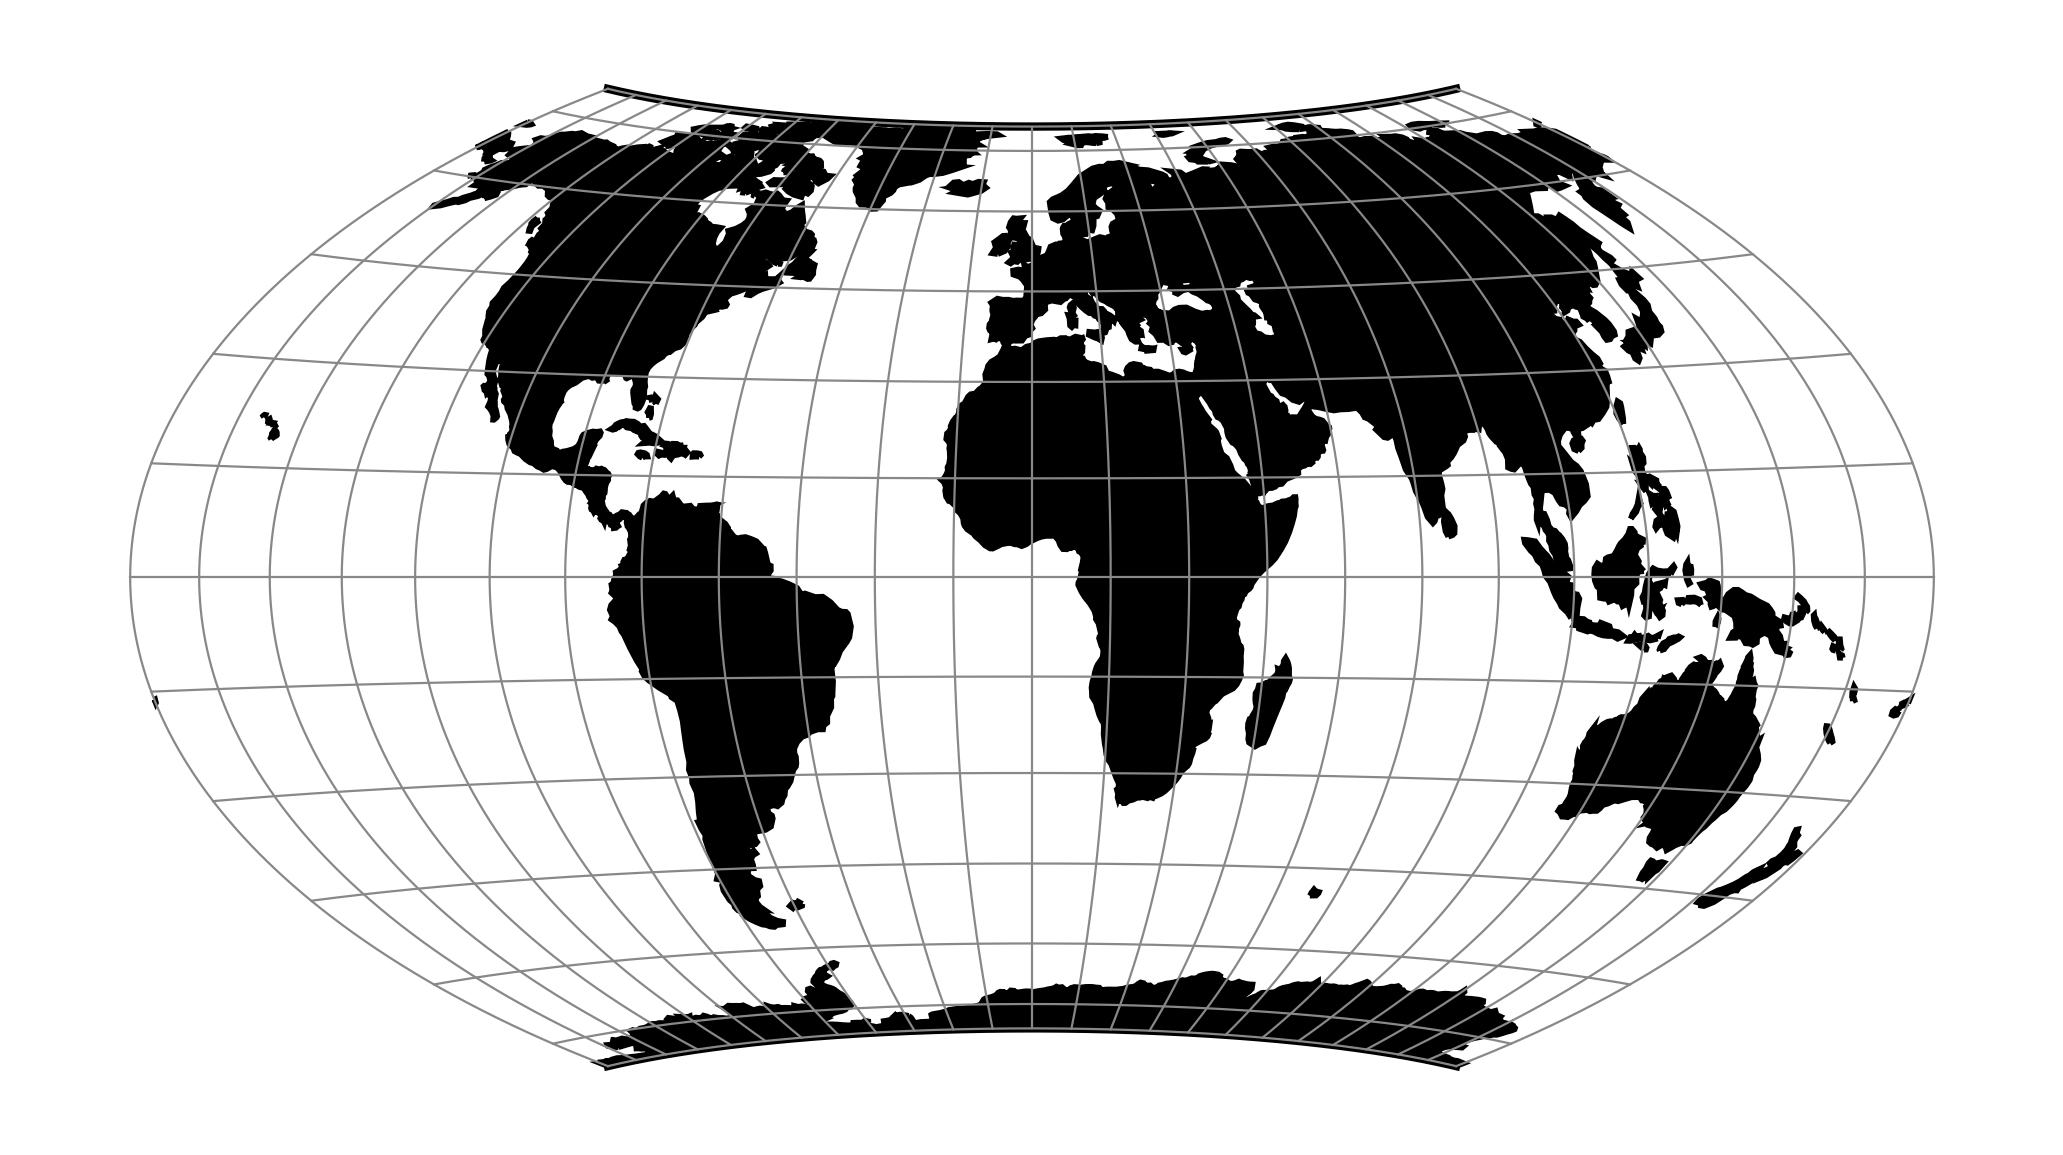
\includegraphics[width=0.9\linewidth]{figures/chapter-8/wag7.png}
        \caption{Wagner VII (Source \cite{PROJ_SITE})}
        \label{fig:wag_proj}
    \end{minipage}\hfill
    \begin{minipage}{0.30\textwidth}
        \centering
        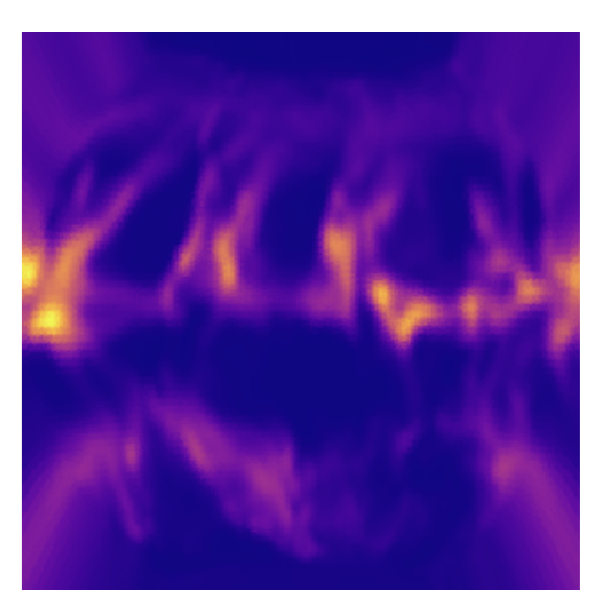
\includegraphics[width=0.9\linewidth]{figures/chapter-8/prect_wag.png}
        \caption{Precipitation raster data as Wagner VII projected}
        \label{fig:wag_prect_raster}
    \end{minipage}\hfill
\end{figure}

\subsection{Results}
